% upon AAS submission
%\documentclass[12pt,twocolumn,tighten,linenumbers]{aastex63}
%\documentclass[12pt,twocolumn,tighten,linenumbers,trackchanges]{aastex63}
% drafting / arxiv
\documentclass[11pt,twocolumn,tighten]{aastex63}
\turnoffedit

\usepackage{apjfonts}
\usepackage{url}
\usepackage{hyperref}
\usepackage{natbib}
\usepackage{amsmath,amstext,amssymb}
\usepackage[caption=false]{subfig} % for subfloat
\usepackage{xcolor, fontawesome}
\usepackage{color}
\usepackage{enumitem}

\newcommand{\red}{\color{red}}

\newcommand{\rprs}{{$R_p/R_{\star}$}}
\newcommand{\vsini}{{$V \sin i$}}
\newcommand{\kms}{{km\,s$^{-1}$}}
\newcommand{\gcc}{{g\,cm$^{-3}$}}
\newcommand{\rstar}{{$R_\star$}}
\newcommand{\rhostar}{{$\rho_\star$}}
\newcommand{\mearth}{{M$_\oplus$}}
\newcommand{\rearth}{{R$_\oplus$}}
\newcommand{\rsun}{{$R_\odot$}}
\newcommand{\msun}{{$M_\odot$}}
\newcommand{\bprp}{G_{\rm BP} - G_{\rm RP}}

\newcommand{\minus}{\scalebox{0.5}[1.0]{$-$}}

%%%%%%%%%%%%%%%%
% INSTITUTIONS %
%%%%%%%%%%%%%%%%
\newcommand{\caltech}{Department of Astronomy, MC 249-17, California Institute of Technology, Pasadena, CA 91125, USA}
\newcommand{\mitkavli}{MIT Kavli Institute and Department of Physics, 77 Massachusetts Avenue, Cambridge, MA 02139}
\newcommand{\berkeley}{Astronomy Department, University of California, Berkeley, CA 94720, USA}

%%%%%%%%%%%%%%%%%%%%%%%%%%%%%%%%%%%%%%%%%%
%%%%%%%%%%%%%%%%%%%%%%%%%%%%%%%%%%%%%%%%%%
%%%%%%%%%%%%%%%%%%%%%%%%%%%%%%%%%%%%%%%%%%

%%%%%%%%%
% STARS %
%%%%%%%%%
\newcommand{\nuniqstarsantosrot}{53{,}663}
\newcommand{\nuniqstarsantosrotgyroappl}{23{,}355}
\newcommand{\nnonfpcumkois}{4{,}716}
\newcommand{\nnonfpcumkoihosts}{3{,}606}
\newcommand{\nplwgyroage}{982}
\newcommand{\nplhoststarwgyroage}{741}
\newcommand{\nplwgyroagenograzing}{767}
\newcommand{\nplhoststarwgyroagenograzing}{585}
\newcommand{\nuniqstarsantosrotteffcut}{45{,}229}
\newcommand{\ratiombtoybstars}{1.4}
\newcommand{\ratioobtoybstars}{2.2}
\newcommand{\ratiombtoybplanets}{2.0}
\newcommand{\ratioobtoybplanets}{2.8}
\newcommand{\nybstars}{3407.6}
\newcommand{\nmbstars}{4563.1}
\newcommand{\nobstars}{7084.3}
\newcommand{\nplyounggyro}{102}
\newcommand{\nplhostsyounggyro}{77}
\newcommand{\nplmidgyro}{200}
\newcommand{\nplhostsmidgyro}{140}
\newcommand{\nploldgyro}{275}
\newcommand{\nplhostsoldgyro}{214}
\newcommand{\nplyounggyrotwosigma}{56}
\newcommand{\nplhostsyounggyrotwosigma}{43}
\newcommand{\nplyounggyrothreesigma}{36}
\newcommand{\nplhostsyounggyrothreesigma}{31}
\newcommand{\nuniqstarsantosallbutruwe}{27{,}922}
\newcommand{\nplwgyroagewithgrazingandhighruwe}{1{,}006}
\newcommand{\nplhoststarwgyroagewithgrazingandhighruwe}{728}
\newcommand{\nplhoststarwgyroagejusthighruwe}{40}
\newcommand{\nlithiumstars}{1{,}464}
\newcommand{\nlithiumplanets}{2{,}174}
%\newcommand{\nlithiumgyrostars}{749}
%\newcommand{\nlithiumgyroplanets}{995}
\newcommand{\nkoisnofp}{4{,}716}
\newcommand{\nhireshours}{304}
\newcommand{\nnonfopkoissomeageinfo}{2{,}461}
\newcommand{\nbergeroverlap}{1{,}623}
\newcommand{\nplyounggyrotwosigmanograzingnoruwe}{39}
\newcommand{\nuniqstarfinitegyroage}{37{,}986}
\newcommand{\fracconsistentallages}{95}
\newcommand{\fracconsistentminageltonegyr}{78}
\newcommand{\allagesyesconsistent}{697}
\newcommand{\allagesmaybeconsistent}{12}
\newcommand{\allagesnoconsistent}{22}
\newcommand{\minageltonegyryesconsistent}{76}
\newcommand{\minageltonegyrmaybeconsistent}{12}
\newcommand{\minageltonegyrnoconsistent}{10}
\newcommand{\fracpotentiallyconsistentallages}{97}
\newcommand{\fracpotentiallyconsistentminageltonegyr}{90}
\newcommand{\nnewdavidtwentyone}{178}
\newcommand{\kepsixsixtgyro}{$1417^{+635}_{-353}$}
\newcommand{\kepsixseventgyro}{$877^{+107}_{-120}$}
\newcommand{\ratiosfr}{2.87}
\newcommand{\uncratiosfr}{0.13}
\newcommand{\trestwotli}{$785^{+845}_{-419}$}
\newcommand{\kepseveneightsix}{$228^{+168}_{-87}$}
\newcommand{\kepsixteenfourfour}{$77^{+144}_{-53}$}
\newcommand{\kepsixteenninenine}{$85^{+106}_{-58}$}
\newcommand{\kepnineteenfourthree}{$409^{+520}_{-254}$}
\newcommand{\allagesqflagyesconsistent}{376}
\newcommand{\allagesqflagmaybeconsistent}{4}
\newcommand{\allagesqflagnoconsistent}{2}
\newcommand{\fracconsistentallagesqflag}{98}
\newcommand{\fracpotentiallyconsistentallagesqflag}{99}
\newcommand{\minageltonegyrqflagyesconsistent}{38}
\newcommand{\minageltonegyrqflagmaybeconsistent}{4}
\newcommand{\minageltonegyrqflagnoconsistent}{2}
\newcommand{\fracconsistentminageltonegyrqflag}{86}
\newcommand{\fracpotentiallyconsistentminageltonegyrqflag}{95}
\newcommand{\ltonegyrhighqconfirmedtwosided}{14}
\newcommand{\ltonegyrhighqconfirmedonesided}{39}
\newcommand{\kepthirteentwelve}{$357^{+75}_{-109}$}
\newcommand{\kepfifteensixone}{$426^{+74}_{-78}$}
\newcommand{\kepsixteentwonine}{$529^{+62}_{-62}$}
\newcommand{\nplwithspec}{2{,}055}
\newcommand{\nstwithspec}{1{,}369}
\newcommand{\nplwithspecandprot}{1{,}170}
\newcommand{\nstwithspecandprot}{797}
\newcommand{\ltonegyrmediumqconfirmedtwosided}{21}
\newcommand{\ltonegyrmediumqconfirmedonesided}{52}
\newcommand{\kepseveneightsixgyro}{$4390^{+243}_{-241}$}
\newcommand{\nconfirmedplyounggyrotwosigmanograzingnoruwe}{31}
\newcommand{\ncandidateplyounggyrotwosigmanograzingnoruwe}{eight}
\newcommand{\njupitershighqconfirmed}{2}
\newcommand{\nminineptuneshighq}{19}
\newcommand{\nsubsaturnshighq}{four}
\newcommand{\nsuperearthshighq}{12}
\newcommand{\nearthshighq}{six}
\newcommand{\njupitershighq}{two}
\newcommand{\nlongperiodhighq}{two}
\newcommand{\mcquillanonlyratiombtoybstars}{1.4}
\newcommand{\mcquillanonlyratioobtoybstars}{1.9}
\newcommand{\mcquillanonlyratiosfr}{2.24}
\newcommand{\mcquillanonlyuncratiosfr}{0.11}
\newcommand{\mcquillanonlyratiombtoybplanets}{0.3}
\newcommand{\mcquillanonlyratioobtoybplanets}{0.3}


% number of stars monitored by Kepler (quoting Santos19/21)
\newcommand{\nkeplerstars}{$\approx$160{,}000}
% fraction of stars with rotation periods, with teff/logg in Berger+20
\newcommand{\fracstarswithprotwithbtwenty}{{$\approx$94\%}}
% complement of above
\newcommand{\fracstarswithprotwithoutbtwenty}{{$\approx$6\%}}

%%%%%%%%%%%
% PLANETS %
%%%%%%%%%%%
% fraction of KOIs that are not FPs with B+20 parameters
\newcommand{\frackoisnofpwithprotwithbtwenty}{{$\approx$92\%}}

%%%%%%%%%%%%%
% OFT-CITED %
%%%%%%%%%%%%%
\defcitealias{2013ApJ...775L..11M}{M13}
\defcitealias{McQuillan_2014}{M14}
\defcitealias{Mazeh_2015}{M15}
\defcitealias{Santos_2019}{S19}
\defcitealias{Santos_2021}{S21}
\defcitealias{Fulton_2018}{F18}
\defcitealias{Berger_2020a_catalog}{B20}

%%%%%%%%%%%%%%%%%%%%%%%%%%%%%%%%%%%%%%%%%%
%%%%%%%%%%%%%%%%%%%%%%%%%%%%%%%%%%%%%%%%%%
%%%%%%%%%%%%%%%%%%%%%%%%%%%%%%%%%%%%%%%%%%

\begin{document}

%\title{Gyrochrone and Lithium Ages for Stars and Planets Observed by Kepler}
%\title{Ages of the Kepler Stars and Planets}
%\title{A Dearth of Young Stars and Planets in the Kepler Field}
\title{Kepler's Demographic Cliff: Ages of Young Stars and Planets in the Kepler Field}

\correspondingauthor{Luke G. Bouma}
\email{luke@astro.caltech.edu}

\received{---}
\revised{---}
\accepted{---}
\shorttitle{Kepler's Demographic Cliff} 

\shortauthors{Bouma et al.}

\author[0000-0002-0514-5538]{Luke~G.~Bouma}
\altaffiliation{51 Pegasi b Fellow}
\affiliation{\caltech}

\author{coauthors, to include but not limited to
Hillenbrand, Howard, Isaacson, Palumbo}

% <250 words
\begin{abstract}
  %Recent analyses of FGK stars in open clusters have revealed how
  %stellar rotation rates and lithium content evolve over the first few
  %billion years.
  %
  Recent analyses of FGK stars in open clusters have helped clarify
  the precision with which a star's rotation rate, and its lithium
  content, can be used as empirical indicators for its age.
  %
  Here we apply this knowledge to stars observed by Kepler.
  %
  Rotation periods are drawn from previous Kepler analyses; lithium
  is measured from new and archival Keck/HIRES spectra.
  %
  We report rotation-based ages for \nuniqstarsantosrotgyroappl\ stars
  and \nplwgyroagenograzing\ planets for which we believe
  gyrochronology is valid; these rotation-based ages are
  roughly an order of magnitude more precise than isochrone ages in
  this sample of FGK stars.
  %
  The independent lithium ages agree with the rotation-based ages for
  $\approx$90\% of cases, suggesting that most of the rotation-based
  ages are not only precise, they are also accurate.
  %However, the timescales of lithium depletion are such that
  %rotation-based ages are more precise for most of our stellar sample.
  %
  Our resulting catalog includes \nplyounggyrotwosigma\ planets
  younger than 1\,Gyr at 2$\sigma$ (\nplyounggyrothreesigma\ planets
  at 3$\sigma$).
  %
  More broadly, we find that the star formation rate in the Kepler
  field has dropped by a factor of \ratiosfr$\pm$\uncratiosfr over the
  past 3\,Gyr, for both planet hosts as well as for the overall
  stellar sample.
  %
  This ``demographic cliff'' has implications for the star formation
  history of our Galaxy, and it helps clarify the relative balance of
  young and old planets that have been detected in transit surveys of nearby
  stars in the Galaxy.
  %
\end{abstract}

\keywords{Stellar ages (1581), Planet hosting stars (1242), Field
stars (2103), Exoplanet evolution (491), Milky Way evolution (1052),}

\section{Introduction}
\label{sec:intro}

Exoplanet science is in an age of abundance, fueled by the discovery
of thousands of worlds orbiting close to their host stars
\citep{Borucki10,2015JATIS...1a4003R}.  Most of these exoplanets are
billions of years old, similar to the Earth.  This fact leaves many
gaps in our knowledge of what exact dynamical and physical processes
produce the observed exoplanet archetypes.    The reason is that
processes such as thermal cooling \citep{2007ApJ...659.1661F},
atmospheric loss \citep{2019AREPS..47...67O}, giant impacts
\citep{2014prpl.conf..595R}, and dynamical instabilities
\citep{2017MNRAS.470.1750I} are expected to be most efficient over
$\approx$10\,Myr to $\approx$1\,Gyr timescales; when we observe most
known exoplanets, these processes are done, and not much is happening.

Finding and characterizing young ($<$1\,Gyr) exoplanets is one 
possible path toward building a timeline for exoplanet evolution.
Informative individual young systems include V1298~Tau, an adolescent
resonant chain of four transiting puffy planets that is a likely
precusor to the compact multiplanet systems \citep{David_2019}, and
HIP~67522, a Jupiter-sized planet with a Neptunian mass
(\citealt{Rizzuto_2020}; Thao et al.~submitted).
% And perhaps also TOI837, now with a uber massive core!
Population-level analyses have similarly suggested differences in the
size distribution of young exoplanets relative to their older
counterparts
\citep{Berger_2020b_rpage,David_2021,Sandoval_2021,2023AJ....166..248C,2024arXiv240303261V}.

Discovering a young planet requires solving two problems: find the
planet, and measure the star's age.  Each problem admits a range of
solutions \citep[e.g.][]{2008Sci...322.1348M,2012ApJ...756L..33Q}.  In
this article we will consider planets previously known from
transits, and infer new stellar ages using rotation and lithium.

To begin, imagine that the age distribution of stars within a few
hundred parsecs of the Sun is uniform between 0 and 10\,Gyr
\citep[e.g.][]{Nordstrom_2004}.  This approximation clarifies the
rarity of young stars: under these assumptions, $\approx$1\% of nearby
stars have $t$$<$100\,Myr, and $\approx$10\% have $t$$<$1\,Gyr.
Entire fields focused on studying forming protoplanets
\citep{2018A&A...617A..44K}, and on watching exoplanets evolve shortly
after disk dispersal \citep[e.g.][]{2022MNRAS.512.5067K}, are thereby
capped in their maximum achievable sample sizes by the tyranny of the
Galactic star formation rate.

Despite the observational challenges, young close-in planet discovery
has done well over the past decade.  This has been primarily enabled
by Kepler, K2, TESS, and Gaia
\citep[e.g.][]{Meibom_2013,Mann_K2_25_2016,Mann_2017,Curtis_2018,Livingston_2018,David_2019,Bouma_2020_toi837,Rizzuto_2020,Plavchan_2020,Newton_2021,Nardiello_2022,Tofflemire_2021,Barber_2022,Bouma_2022a,Bouma_2022b,Zhou_2022,Zakhozhay_2022,Wood_2023}.
The original strategy from around 2010 to 2020 was to focus on stars
with known ages---obvious members of open clusters---and to search
them for transiting planets.  The resulting stellar ages are precise
at the $\approx$10\% level, and planets discovered in this way are
generally assumed to have the same age as the host cluster.  A more
recent development, facilitated by the second Gaia data release, is
the idea that finding transiting planets can often be easier than
finding and characterizing the host stellar association
\citep[e.g.][]{Tofflemire_2021}.

Despite recent advances, the main problem with the ``cluster-first''
approach is that only $\approx$1\% of stars within the nearest few
hundred parsecs are currently associated with their birth cluster
\citep[e.g.][]{Zari_2018,CantatGaudin_2020,Kounkel_2020,Kerr_2021}.
Most nearby sub-gigayear stars are in the field, and are omitted by
cluster-only planet searches.  
One can appreciate the problem by querying NASA's Exoplanet Archive
\citep[NEA;][]{2013PASP..125..989A}
for transiting planets younger than 1\,Gyr.  Imposing reasonable
precision requirements\footnote{For instance $t$$<$1\,Gyr at 2$\sigma$, or else
ages precise to say S/N$=$3.} gives $\approx$50 ``young''
transiting planets at the time of writing.  Most of these planets are
in clusters, and have been discovered by Kepler, K2, or TESS.
However, combined, those surveys have discovered $\approx$5{,}000
planets.  Unless there is a major bias against the discovery of
sub-gigayear old planets (with precisely constrained ages), we would
expect an order of magnitude more young transiting planets to be
known.

This study aims to resolve two main questions.  First, there is the
question of how wrong it is to assume a uniform age distribution for
stars in the galactic thin disk, particularly young stars.  Second,
where are the missing young transiting planets?  Briefly, we will find
that uniform is incorrect by a factor of a few, and that the missing
young transiting planets mostly have imprecise age measurements which
can be improved.

Given that Kepler's primary mission ended in 2013, one might be
forgiven for assuming that the ages of the Kepler planets are already
known.  Of course, they have been studied: \citet{Berger_2020b_rpage}
and \citet{Petigura_2022} for instance calculated isochrone ages for
Kepler Objects of Interest (KOIs).  These ages are most precise for
stars whose luminosities and temperatures separate them from the
main-sequence.  \citet{David_2021} leveraged both isochronal ages from
an earlier analogous study \citep{Fulton_Petigura_2018_cks_vii}, and
used a relative gyrochrone age-ranking approach that sorted stars
based on whether they rotated faster or slower than a gyrochrone age
of $\approx$2.6\,Gyr \citep{Meibom_2015,Curtis_2020}.  These studies
were conducted in the broader context of investigating trends in
exoplanet demographics, which also depend on stellar metallicity and
mass \citep{Petigura_2018}.  These studies offered limited sensitivity
to the ages of the youngest planets, due to the nature of isochronal
dating.

Gyrochronology offers ages precise to $\lesssim$30\% for FGK stars
between 0.5-4\,Gyr, and can also provide useful age limits at earlier
times \citep{Bouma_2023}.  The idea of using a star's spin-down as a
clock is quite old
\citep{Skumanich_1972,Noyes_1984,Kawaler_1989,Barnes03,Mamajek_2008,Angus_2015},
and physics-based models for the spin-down itself can clarify many
aspects of how the stellar winds, internal structure, and magnetic
dynamo all evolve
\citep[e.g.][]{Matt_2015,Gallet_Bouvier_2015,Spada_2020}.  
In the context of Kepler,
empirical models have been previously applied to derive rotation-based
ages for subsets of the Kepler data
\citep{Walkowicz_2013,Reinhold_2015,Angus_2018}.
There have been major improvements since these pioneering studies in:
\begin{enumerate}[label={\it \roman*)}]
  \item The extent of the Kepler Object of Interest catalog, as well
    as our understanding of which of these objects are false
    positives;
  %
  \item Our empirical understanding of how rotation periods of stars
    in open clusters evolve
    \citep[e.g.][]{Curtis_2019_ngc6811,Gillen_2020,Rampalli_2021,Fritzewski_2021,Rebull_2022,Dungee_2022,2023AJ....166...14B};
  %
  \item Our ability to model not only the mean evolution but also the
    intrinsic dispersion in rotation periods as a function of time
    \citep{Bouma_2023}.  
    For Sun-like stars, the new model is broadly consistent with older
    calibrations \citep[e.g.][]{Mamajek_2008}.  However, for late G
    dwarfs and K dwarfs, the age-calibration differs by factors of a
    few;
  %
  \item Our ability to identify binary stars, which can potentially
    problematic for estimates of rotation-based ages.
\end{enumerate}
Today, rotation-based ages for FGK stars below $\approx$4\,Gyr are
empirically tied to the cluster age scale and rotation sequence, and
are limited in precision by the intrisic scatter in the $P_{\rm rot}$
sequences, and in accuracy by systematic uncertainties in the evolving
spin-down rates, and in the cluster ages themselves.  

Beyond improvements in rotation-based ages, recent years have also
yielded improvements in the lithium age scale.
Lithium ages include two qualitatively distinct regimes: depletion
boundary ages derived for M-dwarfs in star clusters, and the less
precise decline-based ages for individual field FGK stars
\citep{Soderblom_2010}.  Here we focus on the latter approach, which
relies on the observation that the Li abundances of
partially-convective stars gradually decline as they age
\citep[e.g.][]{2005A&A...442..615S}.  The theoretical explanation for
this decline is debated
\citep[e.g.][]{1995ApJ...441..865C,2010ApJ...716.1269D,2019MNRAS.485.4052C}
Empirical understanding has however recently improved due to the work
by \citet{Jeffries_2023}, who built a model for how the equivalent
width (EW) of the \ion{Li}{1} 6708\,\AA\ doublet evolves as a function
of stellar effective temperature and age for a set of 6{,}200 stars in
52 open clusters.  Two-sided lithium ages are useful for Kepler (FGK)
stars between $\approx$0.03-0.5\,Gyr, with a strong dependence on
spectral type since the K-dwarfs lose their surface lithium much
faster than G-dwarfs.  The precision of the ages reported by the
\citet{Jeffries_2023} method in this regime are in the range of
0.3-0.5~dex.

We discuss our methods for selecting stellar and planetary samples in
Section~\ref{sec:selection}, and describe
the origin of our adopted stellar parameters other than ages in
Section~\ref{sec:stellarprops}.
We describe and validate our age-dating methods in
Sections~\ref{sec:rotage} and~\ref{sec:liage}.
The population-level trends for both the parent stellar sample and
the planet sample are discussed in Section~\ref{sec:results}.
A few conclusions are offered in Section~\ref{sec:conclusions}.


\section{Selecting the Stars and Planets}
\label{sec:selection}

\begin{figure*}[!t]
  \begin{center}
    \subfloat{
      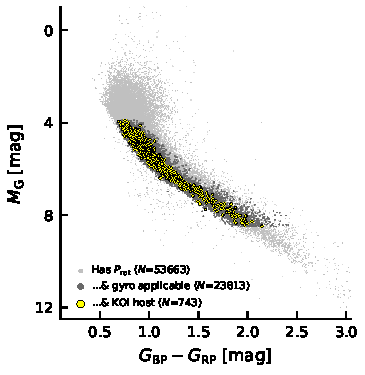
\includegraphics[width=0.49\textwidth]{st_params_M_G_vs_dr3_bp_rp.pdf}
    }
    \subfloat{
    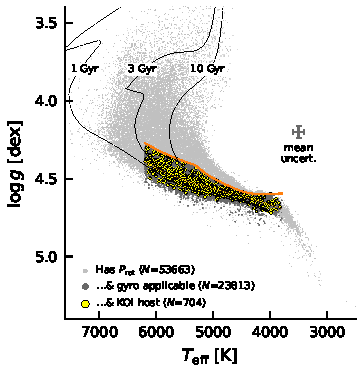
\includegraphics[width=0.49\textwidth]{st_params_adopted_logg_vs_adopted_Teff.pdf}
    }
  \end{center}
  \vspace{-0.5cm}
  \caption{
    {\bf The stars.}  Our analysis focuses on stars observed by Kepler
    with previously reported rotation periods (dark gray points).
    About half of these rotators are suitable for gyrochronology
    (black points), based on factors including their temperatures,
    surface gravities, non-binarity, and proximity to the main
    sequence (see Section~\ref{subsec:flags}).   Some are
    ``confirmed'' or ``candidate'' Kepler Objects of Interest that
    meet an additional set of planetary quality criteria (blue points;
    Section~\ref{subsec:plflags}).  Surface gravities and effective
    temperatures are primarily from \citet{Berger_2020a_catalog}.
  }
  \label{fig:stellarprops}
\end{figure*}

\begin{figure*}[!t]
  \begin{center}
    \leavevmode
    \subfloat{
      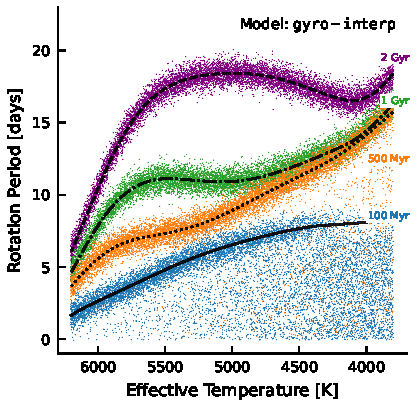
\includegraphics[width=0.49\textwidth]{gyromodeldispersion.pdf}
    }
    \subfloat{
      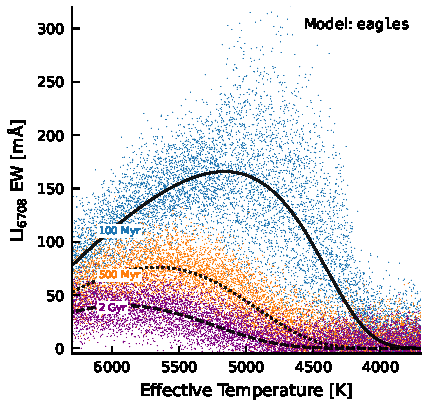
\includegraphics[width=0.49\textwidth]{li_vs_teff_koi_X_S19S21dquality_eagles_showpoints_nodata.pdf}
    }
  \end{center}
  \vspace{-0.6cm}
  \caption{
    {\bf The models.}
    Points represent $10^4$ draws from model probability distributions
    that have been fitted to observed rotation periods
    \citep{Bouma_2023} and lithium equivalent widths
    \citep[EWs;][]{Jeffries_2023} of stars in open clusters.  Lines
    are the ``mean models'' at various ages; the asymmetric intrinsic
    dispersion in rotation and lithium about these mean models, which
    is what the models fit, sets the theoretical precision limit for
    both age-dating methods.    Additional sources of uncertainty,
    including measurement uncertainty, impose further limits on
    achievable age precision.  These models are calibrated using open
    clusters younger than 4\,Gyr.  The displayed points assume a
    uniform distribution in temperature for visual clarity.  The sizes
    of the points are the same in each panel, so that low apparent
    density signifies greater dispersion around the mean.
    \label{fig:models}
  }
\end{figure*}

\begin{figure*}[!t]
  \begin{center}
    \subfloat{
      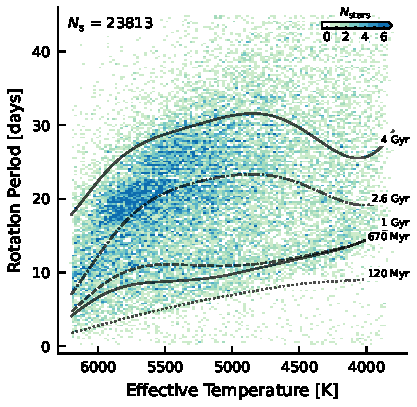
\includegraphics[width=0.48\textwidth]{prot_teff_Santos19_Santos21_dquality.pdf}
    }
    \subfloat{
      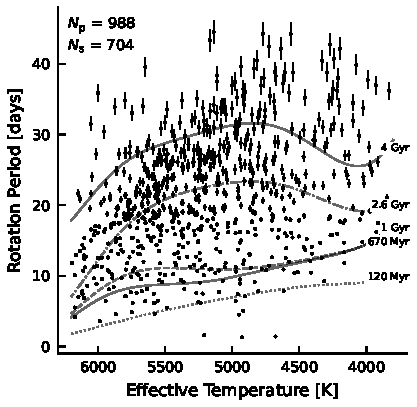
\includegraphics[width=0.48\textwidth]{koi_mean_prot_teff_koi_X_S19S21dquality_keepgrazing.pdf}
    }
  \end{center}
  \vspace{-0.5cm}
  \caption{
    {\bf Rotation periods for Kepler target stars (left) and known
    planet hosts (right)}.  The periods are from \citet{Santos_2019}
    and \citet{Santos_2021} (\citetalias{Santos_2019} and
    \citetalias{Santos_2021}).  The gray lines are ``mean fits'' from
    Figure~\ref{fig:models} to the slow rotation sequences of M67,
    Ruprecht~147, NGC~6811, Praesepe, and a trio of 120\,Myr open
    clusters.  The stellar sample includes only apparently single stars
    near the main sequence with $\log g$$>$4.2, RUWE$<$1.4,
    and 3800$<$$T_{\rm eff}$/K$<$6200.  The displayed planets require
    the same stellar cuts, and include only the confirmed and candidate planets
    described in Section~\ref{subsec:plflags}.
  }
  \label{fig:prot_vs_teff}
\end{figure*}

\begin{figure}[!t]
  \begin{center}
    \leavevmode
    \includegraphics[width=0.49\textwidth]{li_vs_teff_koi_X_JUMP_eagles_logy.pdf}
  \end{center}
  \vspace{-0.6cm}
  \caption{
    {\bf Equivalent widths (EW) of the \ion{Li}{1} 6708\,\AA\ doublet
      for planet-hosting stars.} These measurements were made from
    Keck/HIRES spectra collected between 2009 and 2024 comprising
    \nhireshours\,hours of open-shutter time.  Lines are the ``mean''
    isochrones from the same models as in Figure~\ref{fig:models}; the
    intrinsic dispersion beyond $\approx$1\,Gyr becomes much larger
    than changes in the mean.  The logarithmic scale highlights the
    dynamic range of the detections and upper limits.  Some stars with
    lithium detections do not have detected rotation periods, and
    vice-versa.
    \label{fig:li_vs_teff}
  }
\end{figure}

This work is focused on Kepler stars for which ages can be inferred
using either rotation, lithium, or both.  These ``age-dateable
stars'' are a minority of the \nkeplerstars\ Kepler targets.  Rotation
periods have been reported for roughly one in three Kepler targets
\citep[e.g.][]{McQuillan_2014,Santos_2021}.  High-resolution spectra,
which can yield measurements of the \ion{Li}{1} 6708\,\AA\ doublet, 
have only been acquired for the Kepler objects of interest
(KOIs), which comprise a few percent of Kepler's targets.
In the following, we will describe the set of stars that we
adopt with measured rotation periods (Section~\ref{subsec:rotsel}),
the set of objects we adopt as planets
(Section~\ref{subsec:planetsel}), and the set of planets with
high-resolution spectra suitable for lithium analysis
(Section~\ref{subsec:lithiumsel}).


\subsection{Stellar Rotation Periods}
\label{subsec:rotsel}

To select stars with rotation periods, we turn to previous work.
Many investigators have derived rotation periods both specifically of
the Kepler Objects of Interest
\citep{McQuillan_2013,Walkowicz_2013,Mazeh_2015,Angus_2018,David_2021},
and also of the broader set of all Kepler target stars
\citep{McQuillan_2014,Reinhold_2015,Santos_2019,Santos_2021}.
These studies used a range of detection methods and selection
functions.
We are interested in understanding the age distribution of not only
the KOIs but also the Kepler target stars.
Out of these studies, the only homogeneous analysis of both Kepler
targets and KOIs were the studies by
\citet{Santos_2019} (\citetalias{Santos_2019}),
and \citet{Santos_2021} (\citetalias{Santos_2021}).
\citetalias{Santos_2019} and
\citetalias{Santos_2021} combined a wavelet analysis and
autocorrelation-based approach, and cumulatively reported rotation
periods for 55{,}232 main-sequence and subgiant FGKM stars.
They included known KOIs and binaries in their analysis, and assigned
them specific quality flags, while removing transits and eclipses
during the stellar rotation measurement process. 

%Studies of stellar rotation across the entire Kepler field include
%those by \citet{McQuillan_2014} (\citetalias{McQuillan_2014}),
%\citet{Reinhold_2015}, \citet{Santos_2019} (\citetalias{Santos_2019}),
%and \citet{Santos_2021} (\citetalias{Santos_2021}).
%\citetalias{McQuillan_2014} used an approach based on the
%autocorrelation function to detect 34{,}030 rotation periods for
%main-sequence Kepler targets cooler than 6500\,K, and excluded known
%eclipsing binaries and KOIs.  \citet{Reinhold_2015} used an iterative
%Lomb-Scargle based approach to analyze $\approx$40{,}000 stars with a
%variability range $R_{\rm var}>0.3$\% that were not known EBs, planet
%candidates, or pulsators; they reported primary rotation periods for
%24{,}124 of these stars.  \citet{Reinhold_2015} also reported
%secondary periods for two thirds of the stars with primary periods,
%which could be caused by differential rotation or finite spot
%lifetimes.  Finally, \citetalias{Santos_2019} and
%\citetalias{Santos_2021} combined a wavelet analysis and
%autocorrelation-based approach, and cumulatively reported rotation
%periods for 55{,}232 main-sequence and subgiant FGKM stars.
%\citetalias{Santos_2019} and \citetalias{Santos_2021} included known
%KOIs and binaries, and assigned them specific quality flags.  The
%rotation periods of KOIs have received considerable additional
%scrutiny
%\citep[e.g.][]{Walkowicz_2013,Mazeh_2015,Angus_2018,David_2021}.

We therefore adopt the results of \citetalias{Santos_2019} and
\citetalias{Santos_2021} as our default rotation periods.
\citetalias{Santos_2021} provided a comparison against
\citetalias{McQuillan_2014}; the brief summary is that the periods
agree for 99.0\% of the 31{,}038 period detections in common between
the two studies.  \citetalias{Santos_2021} classified the 2{,}992
remaining stars from \citetalias{McQuillan_2014} as not showing
rotation periods based on updated knowledge of contaminants
(e.g.~giant stars and eclipsing binaries) and visual inspection.  In
addition, \citetalias{Santos_2021} reported rotation periods for
24{,}182 main-sequence and subgiant FGKM stars that were not reported
as periodic by \citetalias{McQuillan_2014}.  Many of these reported
detections have lower variability amplitudes and longer periods than
those reported by \citetalias{McQuillan_2014}.  A relevant flag for
stars missing \citetalias{McQuillan_2014} periods is included in
Table~\ref{tab:stars}.

Analyzing the compilation of \citetalias{Santos_2019} and
\citetalias{Santos_2021} rotation periods for the KOI hosts, we
noticed that some known KOIs with rotation periods were missing.
This is not surprising, in that the rotation periods of KOIs have
received considerably more scrutiny than those of ordinary Kepler
stars.
We therefore decided to split our subsequent analysis into a
homogeneous portion that used only the \citetalias{Santos_2019} and
\citetalias{Santos_2021} data, and an inhomogeneous portion that also
considered a broader set of available KOI rotation periods.
For the latter portion, we first included 32 KOIs with orbital and
rotation periods within $\approx$20\% that had been
excluded\footnote{Excluding stars in this category would impose a bias
against young close-in planets, due to the natural commensurability
between the rotation rates of young stars, and Kepler's increased
sensitivity to short-period objects.  Although some of these KOIs are
known false positives, our analysis excludes such objects at later
steps.}%  As one motivating example, this subset of stars includes {\it
%e.g.}~Kepler~1643 (KIC~8653134), with $P_{\rm orb}$=5.34\,days and
%$P_{\rm rot}$=5.05\,days, which is known to be $\approx$40\,Myr old
%based on membership in RSG-5 \citep{Bouma_2022b}.  }
from the
\citetalias{Santos_2019} and \citetalias{Santos_2021} catalogs
(A.~Santos, private communication).
We then incorporated an additional \nnewdavidtwentyone\ rotation
periods for KOI hosts that
\citet{David_2021} had described as either ``reliable'' or ``highly
reliable'' in their visual analysis of previously reported KOI
rotation periods from \citet{McQuillan_2013,Walkowicz_2013,Mazeh_2015}
and \citet{Angus_2018}.
Inclusion of these additional KOI rotation periods is a
supplementary measure aimed at completeness in our final KOI age
catalog; the provenances of the individual adopted periods are all
noted in the relevant tables.

Finally, since our scope is focused on rotation-based age dating, 
we restricted our attention to stars with reported $P_{\rm
rot}$$<$45\,days.
FGK stars with slower rotation periods spin much slower than the stars
in the oldest open clusters currently used to calibrate empirical
gyrochronal models.

The resulting tally of stars from
\citetalias{Santos_2019}, \citetalias{Santos_2021}, and our corrected
KOI list is \nuniqstarsantosrot\ Kepler stars with rotation periods.

As a sanity check on the statistical uncertainties of these rotation
periods, we compared our adopted \citetalias{Santos_2019} and
\citetalias{Santos_2021} periods with those reported by
\citet{McQuillan_2014} and \citet{Mazeh_2015}.  We found that for
$P_{\rm rot}\lesssim$15\,days, the two datasets agree at a precision
of $\lesssim$0.01$P_{\rm rot}$.  At longer periods of $P_{\rm
rot}\approx$30\,days, the agreement was typically at the
$\lesssim$0.03$P_{\rm rot}$ level, and the upper envelope of the
period difference increased roughly linearly with period.  Based on
this comparison, we adopted a simple prescription for the period
uncertainties, such that there are 1\% relative uncertainties below
$P_{\rm rot}=15$\,days, and a linear increase thereafter, with slope
set to guarantee 3\% $P_{\rm rot}$ uncertainties at rotation periods
of 30 days.


\subsection{Kepler Objects of Interest}
\label{subsec:planetsel}

We considered planets in the NASA Exoplanet Archive's cumulative KOI
table, which included the best knowledge available on any given planet
candidate as of 6 June 2023, while also incorporating human-based
vetting.\footnote{See
\url{https://exoplanetarchive.ipac.caltech.edu/docs/PurposeOfKOITable.html}}
These planets represent a superset of those in the fully automated
Q1-Q17 DR25 KOI Table \citep{Thompson_2018}, which could be adopted in
future work for planet occurrence rate calculations.  This version of
the cumulative KOI table included \nkoisnofp\ objects that are either
``confirmed'' or ``candidate'' planets, after excluding known false
positives. 

\subsection{High Resolution Spectra}
\label{subsec:lithiumsel}

The final piece of our analysis involves assessing ages based on the
equivalent width of the \ion{Li}{1} 6708\,\AA\ doublet.  Specifically,
we analyzed spectra acquired with the High Resolution Echelle
Spectrometer (HIRES; \citealt{vogt_hires_1994}) on the Keck I 10m
telescope.  These spectra were primarily collected through the
California Kepler Survey
\citep{2017AJ....154..107P,2017AJ....154..108J,2017AJ....154..109F}.
We supplemented the existing archive with $\approx$10~hours of new
observations for 22 stars between Fall 2022 and Spring 2024.  These
stars were chosen to ensure that confirmed planets with rotational
evidence for ages below 1\,Gyr had spectra, since this is the age
range in which lithium is most likely to yield useful age constraints.

% stat from _estimate_new_lithium_timefrac.py
Lithium equivalent widths and abundances for the Kepler Objects of
Interest were already analyzed by \citet{2018ApJ...855..115B} for
about three quarters of the spectra in our sample.  However, since new
spectra have been acquired since the \citeauthor{2018ApJ...855..115B}
analysis, and since our approach and selection function are different,
we opt to perform our own analysis of the reduced HIRES spectra.

We queried the internal CPS archive to collect all blaze-corrected
HIRES spectra that were available for all non-false positive Kepler
Objects of Interest with a MES$>$10.  This query yielded at least one
spectrum for \nlithiumstars\ stars and \nlithiumplanets\ planets.  For
stars with multiple spectra available at varying ranges of
signal-to-noise (S/N), we analyzed only the spectrum with the highest
number of counts.  The resulting spectra were acquired between 6
September 2009 and 16 May 2024, and cumulatively comprise
\nhireshours\,hours of open-shutter time.

We measured the lithium equivalent widths using a procedure
adapted from previous work \citep{Bouma_2021}.  Our stars of interest
are FGK stars, and so the continuum in the vicinity of the \ion{Li}{1}
6708\,\AA\ doublet is well-defined.  We Doppler corrected the spectra
to a common reference wavelength by cross-correlating against a high
S/N template for Kepler-1698, chosen because $\gamma$$\approx$9\kms,
$T_{\rm eff}$$\approx$5000\,K and $v\sin i$$\approx$5\,\kms, which
puts it in the middle of our sample's temperature range and gives it
mild line-broadening.  We then trimmed the Doppler-corrected spectra
to a local window centered on the lithium line, using a window width
of 15\,\AA\ (we considered 10\,\AA\ and 20\,\AA; the results were
broadly consistent).  We continuum-normalized by fitting a
third-degree Chebyshev series, while excluding regions with
absorption lines.  We then numerically integrated the resulting
spectrum using a one-component Gaussian with free amplitude, width,
and mean, and estimated uncertainties on the line width through a
Monte Carlo procedure that bootstraped against the local scatter in
the continuum.

Our EW measurement approach does not correct for the neighboring
\ion{Fe}{1} 6707.44\,\AA\ blend.  To evaluate the accuracy and
precision of our equivalent measurement technique, after applying an
initial iteration on the \nlithiumstars\ KOIs with spectra, we
compared our lithium equivalent widths with those reported by
\citet{2018ApJ...855..115B}.  For the \nbergeroverlap\ stars in both
samples, we found broad agreement at $>$30\,m\AA, and significant
differences at $<$30\,m\AA because \citet{2018ApJ...855..115B}
required positive EWs, while we allow for negative ones.  At
$>$30\,m\AA, there is however a small offset in our respective
scales, such that (B24-B18)$=$7.50$\pm$8.55\,m\AA.  This offset is
caused by our non-treatment of the iron blend.  We therefore directly
subtract the constant mean value noted above when calculating
lithium-based ages.




\section{Stellar Properties}
\label{sec:stellarprops}

% https://gea.esac.esa.int/archive/documentation/GDR3/Data_analysis/chap_cu8par/sec_cu8par_apsis/ssec_cu8par_apsis_gspphot.html

Our default source for stellar temperatures and surface gravities is
the Gaia-Kepler Stellar Properties Catalog (GKSP;
\citealt{Berger_2020a_catalog}).  The GKSP parameters were reported
for stars with ``AAA'' 2MASS photometry, measured parallaxes in Gaia
DR2,  and $g$-band photometry from either the KIC or the Kepler-INT
survey.  The parameters themselves were derived using
\texttt{isoclassify} \citep{2017ApJ...844..102H} to interpolate over
the MIST isochrone grids
\citep{2016ApJ...823..102C,2016ApJS..222....8D}, given the SDSS $g$
and 2MASS $K_{\rm s}$ photometry, the Gaia DR2 parallaxes, and
$V$-band extinction from the \citet{2018MNRAS.478..651G} reddening
map.  The resulting stellar parameters are available for
\fracstarswithprotwithbtwenty\ of the \nuniqstarsantosrot\ Kepler
stars with rotation periods.  For the remaining
\fracstarswithprotwithoutbtwenty\ of stars that lack temperatures and
surface gravities from \citetalias{Berger_2020a_catalog}, we adopt the
values reported by \citet{Santos_2019} and \citet{Santos_2021}, which
for these cases primarily derive from the \citet{Mathur_2017} DR25
Kepler Stellar Properties Catalog, and are mostly derived from
photometry.  In the planet sample, \frackoisnofpwithprotwithbtwenty\
of the non-false-positive KOIs with rotation periods have parameters
from \citet{Berger_2020a_catalog}, and the remainder similarly are
drawn from DR25. 

\citet{David_2021} compared the photometric
\citetalias{Berger_2020a_catalog} stellar parameters ($T_{\rm eff}$,
$R_\star$, [Fe/H]) against the spectroscopic parameters from
\citet{Fulton_2018}.  The temperature scales did show a few-percent
systematic difference, with \citetalias{Fulton_2018} quoting higher
temperatures than \citetalias{Berger_2020a_catalog} for mid K dwarfs,
and lower temperatures for early F dwarfs.  Our age analysis,
described below, assumes Gaussian uncertainties in effective
temperatures; we by default adopt the maximum of the two-sided
uncertainties reported by \citetalias{Berger_2020a_catalog} as our
symmetric temperature uncertainty.  Overall, the impact of systematic
uncertainties in the temperature scale on our age uncertainties is
generally smaller than that of the intrinsic scatter in the
calibration sequences of the open clusters.

% optional todo's:
%TODO: plot uncertainties in teff vs teff...
%TODO: plot uncertainties in logg vs logg...
%TODO: add that plot showing differences btwn the two teff scales?




\section{Ages From Rotation}
\label{sec:rotage}

We calculate gyrochrone ages using \texttt{gyro-interp}
\citep{Bouma_2023}, which is a method designed to address the issue
that, especially over the first gigayear of stellar spin-down, stars
with the same mass and same rotation period can have very different
ages \citep[e.g.][]{Curtis_2019_ngc6811}.  The gyrochrone age
posterior should therefore incorporate this intrinsic population-level
scatter into the precision with which the age can be inferred.
Figure~\ref{fig:models} highlights this problem, particularly in
regions where the 0.1-1\,Gyr stars overlap.

Using our adopted effective temperatures and rotation periods, we ran
\texttt{gyro-interp} over an age grid of 0 to 4\,Gyr, linearly spaced
over 500 grid points.  \texttt{gyro-interp} itself is calibrated out
to 4\,Gyr, the age of M67
\citep[see][]{2022ApJ...938..118D,Gruner_2023}.  To estimate the
stellar spin-down rate as a function of time and stellar temperature,
the framework interpolates between reference open clusters using
smooth cubic hermite polynomials.  We calculate the probability of the
rotation-based age $t_{\rm gyro}$, given the observed rotation
periods, effective temperatures, and their uncertainties by
integrating Equation~1 of \citet{Bouma_2023} at the default grid
resolution.  This procedure marginalizes over the intrinsic age and
temperature dependent scatter that is observed in the cluster
sequences to yield statistical age uncertainties.


\subsection{Gyrochronology Quality Flags}
\label{subsec:flags}
We calculated gyrochrone age posteriors for all
\nuniqstarsantosrotteffcut\ stars with reported rotation periods and
effective temperatures between 3800\,K and 6200\,K.  To flag stars for
which we suspect these ages may not in fact be valid, we built a set
of bit-quality flags.  When and how these flags should be applied
depends on the question being asked.  If the goal is to construct a
false-positive free sample, they might all be applied.  If the goal is
to construct a complete sample of young stars, then consider the
examples of Kepler~1627Ab ($\approx$40\,Myr) and Kepler~51c
($\approx$625\,Myr).  The former has a high RUWE due to a resolved
binary companion \citep{Bouma_2022a}; the latter is on a grazing orbit
\citep{2014ApJ...783...53M}.  Our gyrochronology quality flag, $Q_{\rm
gyro}$, enables selecting for or against such cases by selecting from
the following bits.

As a general philosophy, three assumptions must hold for a
rotation-based age dating method like \texttt{gyro-interp} to be
valid.  {\it 1)} The evolutionary state of the target star must be
well-specified by its temperature and its age, {\it 2)} the star's
spindown must not be influenced by binary companions, and {\it 3)} the
rotation period distribution for field stars of a given temperature
and age must be identical to that of equally aged open clusters
(metallicity differences, for instance, are ignored).  A rephrasing of
the first condition is that the star must be ``near the main
sequence'', because during post main sequence evolution, the
temperatures of stars change.  From $\approx$0.08 to $\approx$3\,Gyr,
the stars of interest in this work (3800--6200\,K,
0.5--1.2\,$M_\odot$) have temperatures constant to $\approx$1\%
\citep{Choi_2016}.  From $\approx$3--4\,Gyr, a 1.2\,$M_\odot$ star's
temperature drops from $\approx$6200\,K to $\approx$6000\,K
($\approx$3\%), because its outer layers expand as it begins hydrogen
shell burning as a subgiant.  We treat this issue in a somewhat
convoluted manner, discussed in ``bit 9'' below.

{\it Temperature range (bit 0)}---We require stars to have effective
temperatures $T_{\rm eff}$ between 3800 and 6200\,K in order to report
gyrochrone ages \citep{Bouma_2023}.   Stars hotter than 6200\,K spin
down very slowly, if at all.  Stars cooler than 3800\,K do spin down
over gigayear timescales
\citep{2016ApJ...821...93N,2023ApJ...954L..50E,2024arXiv240312129C},
but the currently available open cluster data have yet to clarify
exactly when the intrinsic scatter in the population decreases.

{\it Surface gravity (bit 1)}---We flagged stars as possible subgiants
if they had $\log g < 4.2$.  We set this threshold by examining the
relevant flag from \citet{berger_2018_radii_evolnstates},
cross-matched against \citet{Berger_2020a_catalog}.

{\it Absolute luminosity (bit 2)}---We calculated the absolute Gaia
DR3 $G$-band luminosity, ignoring reddening, using the reported
apparent $G$-band magnitude and parallaxes.  We flag stars with
$M_{\rm G} < 3.9$ or $M_{\rm G} > 8.5$, corresponding to main-sequence
spectral types earlier than $\approx$F8V or later than $\approx$M0.5V
\citep{Pecaut_2013}.

{\it Known eclipsing binaries (bit 3)}---We flagged any stars reported
to be in the final Kepler eclipsing binary catalog (KEBC;
\citealt{2016AJ....151...68K}).

{\it Kepler-Gaia crossmatch quality (bits 4 and 5)}--- In situations
where we wanted to leverage Gaia DR3 data, we used M.~Bedell's 4$''$
Kepler-to-Gaia crossmatch\footnote{\url{https://gaia-kepler.fun}, last
accessed 15 April 2024.  We used 4$''$ rather than the 1$''$ match
because 91 KOIs are omitted in the 1$''$ match, 23 of which have
either ``candidate'' or ``confirmed'' status.  Almost all of these 23
are M dwarfs with high proper motions.  Performing the same crossmatch
at 4 arcseconds, only two KOIs (KOI-3993 and KOI-6531), both known
false positives, fail to yield Gaia DR3 crossmatches.}, which is a
crossmatch of the NASA Exoplanet Archive
\texttt{q1\_q17\_dr25\_stellar} catalog with Gaia DR3.  The separation
distribution of the Kepler-Gaia DR3 crossmatches is such that 99.2\%
of candidate matches are within 1$''$.   We nonetheless noted an
upturn in the candidate match rate from 3-4$''$; such sources are
flagged using bit 4.  For KIC stars with multiple potential Gaia
matches within the 4$''$ search radius, we adopted the brightest star
as the default match.  In most such cases this was unambiguous because
there is a large brightness difference between the primary and any
apparent neighbors.  However cases with multiple stars within 4$''$
within $\Delta G$$<$$0.5$\,mag are noted using bit flag 5.  

{\it Gaia DR3 non-single-stars (bit 6)}---The Gaia DR3
\texttt{non\_single\_star} column in the \texttt{gaia\_source} table
flags known eclipsing, astrometric, and spectroscopic binaries.  We
directly include this column.

{\it RUWE (bit 7)}---We inspected diagrams of the Gaia DR3 renormalized
unit weight error
(RUWE) as a function of other stellar parameters, %\footnote{\url{https://gea.esac.esa.int/archive/documentation/GDR3/Gaia_archive/chap_datamodel/sec_dm_main_source_catalogue/ssec_dm_gaia_source.html}})
and flag stars with RUWE$>$1.4 as possible binaries.  Such astrometric
outliers can be either bona fide astrometric binaries, or more often
are marginally resolved point sources for which the single-source PSF
model used in the Gaia pipeline induces spurious astrometric scatter.

{\it Crowding (bit 8)}---We searched the Gaia DR3 point source catalog
for stars within 1 Kepler pixel (4$''$) of every target star.  While
many such companions are not physically associated with the target
star, their presence can bias stellar parameters and stellar rotation
period measurements.  We therefore flag any stars with neighbors down
to 10$\times$ the brightness of the target star within this region
($\Delta G < 2.5$).

{\it Near the main-sequence (bit 9)}---Many stars observed by Kepler
are far from the main sequence: this can be seen in color--absolute
magnitude diagrams, and in diagrams of e.g.~surface gravity as a
function of temperature (Figure~\ref{fig:stellarprops}).  This is a
challenge for rotation-based age-dating because {\it i)} point sources
far from the main-sequence include unresolved photometric binaries,
and {\it ii}) effects other than magnetic braking influence the
rotation periods of bona fide single stars far from the main-sequence.
The added complications of reddening and metallicity make defining a
simple cut in any two dimensions challenging.  
We explored various options, and settled on the orange locus in the
$\log g$--$T_{\rm eff}$ plane shown in Figure~\ref{fig:stellarprops}.
While the details of how exactly this locus is constructed are
arbitrary and convoluted,\footnote{In practice, for K dwarfs we fitted an
$N^{\rm th}$-order polynomial to the set of stars for which $t_{\rm
B20,iso}/(+\sigma_{t,{\rm B20,iso}})\approx 3$, where
$t_{\rm B20,iso}$ was the isochronal age reported by
\citet{Berger_2020a_catalog}. We let the order of the fit vary from
$N$=1 to 10, minimized the Bayesian Information Criterion,
and found $N$=6.  For F and G dwarfs, this procedure failed to produce
a reasonable locus because of shifts in the relative precision of
the isochrone ages.  We therefore visually selected KOIs that appeared
to be near the ``main sequence'', fitted a separate polynomial to
their locations, and then stitched the resulting polynomials from the
F and G dwarfs to that of the K dwarfs.} the general 
aim is to exclude stars for which there is photometric evidence
that gyrochronology may not be reliable.  The rotation period
distribution of sources excluded in this manner includes a relatively
larger fraction of ``rapid rotators'' than the main sequence sources,
likely due to a combination of astrophysical and systematic effects.
See for instance Figure~8a of \citet{2022AJ....164..137K} or Figures~12 and 13
of \citet{2023ApJS..268....4F}.


{\it Candidate pulsators and close-in binaries (bit
10)}---\citeauthor{Santos_2021} included in a flag for candidate
``classical pulsators'' (e.g.\ RR~Lyrae, Cepheids) and candidate
close-in binaries.  Visual inspection of the rotation periods as a
function of temperature shows that although this flag selects many
bona fide objects in these classes, it also selects the overwhelming
majority of $\lesssim$5\,day bona fide young planets.  In our view this is
erroneous because they these objects are neither classical pulsators nor
close binaries.  While we
propagate this flag into our set of quality flags, we therefore
generally ignore it.

{\it How do we use the bit-flags}
An important decision for our subsequent analysis is how to combine
the above quality indicators in order to decide whether or not a star is suited for
gyrochronology.  By default, we assume that a star is suitable for
gyrochronology if none of bits zero through nine (inclusive) are
raised.


\subsection{Planet Quality Flags}
\label{subsec:plflags}
Not all planets are born equal.
We use the following additional quality indicators to assess 
the reliability and utility of a planet, and assemble them into a separate bit-flag,
$Q_{\rm planet}$.

% see Erik's 2022 discussion; might want to shift to include a cut on
% disposition score.
{\it Candidate reliability (bit 0)}---The NEA's Kepler Objects of Interest Table
includes both an overall planet-candidate disposition status
({\it koi\_disposition}), as well as a disposition based only on the Kepler
data ({\it koi\_pdisposition}).
We require both to include only
``planet candidates'' and ``confirmed planets''; we are generally less interested
in the age distribution of planet candidates that are known false positives.

{\it Candidate S/N (bit 1)}---In any transit survey, the false positive rate increases
greatly toward the noise floor for planet detection \citep[e.g.][]{2002ApJ...564..495J}.  We
required a S/N in excess of Kepler's usual 7.1$\sigma$ floor, through a cut on the
maximum
``multiple event statistic'' (MES, {\it koi\_max\_mult\_ev}): we required ${\rm MES}$$>$10.

{\it Grazing planets (bit 2)}---Grazing objects, for which the impact
parameter $b$ is greater than $1-R_{\rm p}/R_\star$,
often yield biased planetary parameters
\citep[e.g.][]{2022AJ....163..111G}.
Particularly for large planets, they can also include
astrophysical false positives at higher rates \citep{2016ApJ...822...86M}, which is
in part due to the size-impact parameter degeneracy.
We flag planet candidates as potentially grazing if $b>0.8$, 
using the impact parameters reported in the Markov Chain
Monte Carlo (MCMC) fits from \citet{Thompson_2018}.


\subsection{Sample Summary}
\label{subsec:tally}

The rotation periods for the stellar and planetary samples are shown
in Figure~\ref{fig:prot_vs_teff}.  Out of the \nkeplerstars\ stars
observed by Kepler, requiring reported rotation periods and a reliable
DR3 crossmatch yielded \nuniqstarsantosrot\ stars.  Further requiring
these rotating stars to have temperatures 3800$<$$T_{\rm
eff}$/K$<$6200, which is the range over which \texttt{gyro-interp}
returns finite age posteriors, yields \nuniqstarsantosrotteffcut\
stars.  Further requiring the stars to be apparently single, near the main
sequence, with $\log g$$>$4.2, $M_{\rm G}>3.9$, and not flagged as
eclipsing binaries yielded \nuniqstarsantosallbutruwe\ rotators
potentially amenable for gyrochronology.  Finally, imposing RUWE$<$1.4
and requiring no possible blends ($\Delta G$<2.5) within 4$''$ leaves
\nuniqstarsantosrotgyroappl\ stars for which gyrochronology is likely
to be valid.


In the planet sample, the cumulative KOI table included
\nnonfpcumkois\ confirmed and candidate planets, orbiting
\nnonfpcumkoihosts\ stars.  Assume that we apply all the same stellar
cuts, save for that on RUWE.  Then, require these confirmed and
candidate planets to have MES$>$10.  This combination of selection
criteria yield \nplwgyroagewithgrazingandhighruwe\ planets with
rotation-based ages orbiting
\nplhoststarwgyroagewithgrazingandhighruwe\ stars
(\nplhoststarwgyroagejusthighruwe\ of these stars with ``high'' RUWE).
If we additionally require the planets to be non-grazing ($b<0.8$),
we are left with \nplwgyroagenograzing\ planets orbiting
\nplhoststarwgyroagenograzing\ stars.




\section{Ages From Lithium}
\label{sec:liage}


Figure~\ref{fig:li_vs_teff} shows our measured equivalent widths for
the lithium 6708\AA\ absorption doublet, plotted over the mean
isochrone models from \texttt{EAGLES} \citep{Jeffries_2023}.  We
declare an upper-limit for plotting purposes if the 1$\sigma$ lower
limit on the equivalent width is below 10\,m\AA.  Our measured EWs
span -40 to 250\,m\AA; all negative EWs have uncertainties that are
statistically consistent with zero.

To calculate lithium ages, we use \texttt{EAGLES} (git commit
\texttt{ac09637}), which, similar to
\texttt{gyro-interp}, is based on a purely empirical interpolation
approach.  \texttt{EAGLES} however was calibrated on lithium measurements of
stars observed by the
Gaia-ESO spectroscopic survey in 52 open clusters with ages spanning 2
to 6{,}000\,Myr \citep{Jeffries_2023}.  We adopt a linear prior in
age, spanning $10^6$ to $10^{10}$\,yr, and symmetrize our EW
uncertainties for purposes of interfacing with \texttt{EAGLES} by
taking the maximum of the measured positive and negative 1$\sigma$
uncertainty intervals.
Certain quality flags described in Section~\ref{subsec:flags} are also
relevant for lithium ages, specifically those associated with
crowding and binarity.
For instance, rapid rotators are more common in binaries, and they also
generally have higher lithium abundances than slow-rotating stars of the
same mass (CITE).
Stars for which rotation-based age dating is dubious heavily overlap
with those for which lithium-based ages are dubious.

In part because many of our EWs are upper limits, 
many of the lithium ages are lower limits.
In such cases,  the inferred age posterior is strongly influenced by
{\it i)} the assumed intrinsic dispersion in the lithium model,
and {\it ii)} by the prior.
For instance, 
 we quote the 3$\sigma$ (99.7$^{\rm th}$ percentile) limits.


\section{Results}
\label{sec:results}

\begin{figure*}[!t]
  \begin{center}
    \leavevmode
    \includegraphics[width=\textwidth]{hist_samples_koi_gyro_ages_hist_field_gyro_ages_20240430_maxage3200.pdf}
  \end{center}
  \vspace{-0.6cm}
  \caption{
    {\bf Kepler's demographic cliff,} visible in the rotation-derived
    ages of stars (left) and planet hosts (right) in the Kepler field.
    The lightly colored histograms correspond to all
    \nuniqstarsantosrotteffcut\ $T_{\rm eff}\in[3800,6200]\,$K Kepler
    stars with reported rotation periods, and all
    \nplhoststarwgyroage\ planet-hosting stars with reported rotation
    periods.
    The darker histograms impose the necessary quality cuts on factors
    such as binarity, crowding, and the star's evolutionary state
    (Section~\ref{subsec:flags}).
    In detail, these ``histograms'' are resampled from the posterior
    probability distributions, and so have less resolution at
    $\lesssim$0.5\,Gyr, when the relative precision of rotation-based
    ages decreases.
    Completeness is near unity at t$\lesssim$3\,Gyr
    \citep{2022ApJ...937...94M}.
    {\bf todo: numbers dont match.  why?}
    \label{fig:hist_tgyro}
  }
\end{figure*}

\subsection{The Demographic Cliff}

Figure~\ref{fig:hist_tgyro} shows the gyrochone age distributions of
stars and planet-hosts in the Kepler field.  We truncated the plots
near $3$\,Gyr due to arguments that suggest the detectability of
rotation signals is near-unity up to this age for Sun-like stars, and
decreases for older ages \citep{2022ApJ...937...94M}.  Both the
stellar and planetary samples point toward a star formation rate in
the Kepler field that has slowed over the past few gigayears.

Imagine we were to group stars between 0-1\,Gyr, 1-2\,Gyr, and
2-3\,Gyr, and label them ``young'', ``intermediate-age'', and ``old''.
A simple counting exercise from the distributions in
Figure~\ref{fig:hist_tgyro} tells us that there are \ratioobtoybstars\
times as many old stars in the Kepler field as young stars.
Similarly, there are \ratioobtoybplanets\ times as many old planet
hosts as young planet hosts. 

In terms of detected planet counts, our rotation-based ages for the
Kepler sample yield \{\nplyounggyro, \nplmidgyro, \nploldgyro\}
detected planets in the 0-1\,Gyr, 1-2\,Gyr, and 2-3\,Gyr bins.  For
the sub-gigayear bin in particular, which holds specific weight in
studies of planet evolution, while there are \nplyounggyro\ planets
with median ages below 1\,Gyr, requiring $t_{\rm gyro}$$<$1\,Gyr at
2$\sigma$ confidence yields \nplyounggyrotwosigma\ planets orbiting
\nplhostsyounggyrotwosigma\ stars.  The stellar and planetary
properties of this latter sample of young planets are given in
Table~\ref{tab:planets}.


\subsection{Planets Younger Than One Billion Years}

Given that the history of young exoplanet discovery includes a
sociological tendency to report detailed descriptions of specific
young exoplanets, we find it necessary to briefly discuss the
properties of at least the most notable members of the set of
confirmed planets that have well-measured ages.  We first focus on
systems reported to be in the four stellar ensembles in the Kepler
field that have yielded transiting planets: Cep-Her, MELANGE-3,
Theia~520, and NGC~6811.  We then consider the broader set of Kepler
planets that are young based on the rotational and lithium-based
properties of their host stars.


\subsubsection{Planets in Clusters}
\label{subsec:clusterplanets}

\paragraph{Cep-Her}
Kepler-1627Ab, Kepler-1643b, Kepler-1974b and Kepler-1975\,Ab are
known members of the $\approx$40\,Myr old Cep-Her association
\citep{Bouma_2022a,Bouma_2022b}.  The age of various sub-components of
this association are best measured through relative isochronal
placement of the pre-main-sequence \citep[see][]{Bouma_2022b}, and
gyrochronology of stars in these clusters show them to be $<$100\,Myr
old.  The planets themselves are all on close-in orbits (5-25\,days),
with sizes from 2-4\,$R_\oplus$.  For Kepler-1627A and Kepler-1974,
the rotation, lithium, and cluster-based ages all agree within
1$\sigma$.  For Kepler-1643, while the rotation and cluster ages agree
($46^{+9}_{-7}$\,Myr; \citealt{Bouma_2022b}), the lithium-based age
($198^{+98}_{-76}$\,Myr) is 2.0$\sigma$ above the nominal cluster age
for RSG-5.  For Kepler-1975Ab (KOI\,7913Ab), the lithium age may be
similarly ``old'', though with less confidence due to the large
intrinsic scatter in K dwarf lithium calibration measurements.  For
that system, the isochronal age of its binary companion provides a
more stringent and serendipitous constraint on the $\approx$40\,Myr
age.

\paragraph{MELANGE-3}
\citet{2022AJ....164...88B} described an association in the Kepler
field that was argued to be $105\pm10$\,Myr based on a combination of
rotation, lithium, and the isochronal pre-main-sequence.  Kepler-970
and Kepler-1928 harbor two transiting mini-Neptunes inside this
association \citep{2022AJ....164...88B}.  Our rotation-based
age-dating independently recovers these systems, with $t_{\rm
gyro}=176_{-40}^{+120}$\,Myr and $144_{-88}^{+104}$\,Myr for
Kepler-970 and -1928 respectively.  The former rotation-based age
being slightly older than the suggested Pleiades age for the
assocation agrees with Figure~4 of \citet{2022AJ....164...88B}, where
the MELANGE-3 rotational isochrone is visually slower than
the corresponding Pleiades track.

\paragraph{Theia~520}
Kepler-968 and Kepler-52 both have rotation-based ages of
330-350\,Myr.  These stars were independently reported by
\citet{2019AJ....158..122K} to be members of an association dubbed
Theia~520 based on their spatial and kinematic correlations with
nearby stars.  While the core of this structure was previously named
UBC-1 \citep{2018A&A...618A..59C}, both Kepler planet hosts are in
more diffuse regions of the cluster reported by
\citet{2019AJ....158..122K}, so we adopt the name from the latter
study.  The nominal age of Theia~520 reported by
\citet{2019AJ....158..122K} based on isochrone fitting was
$247^{+64}_{-51}$\,Myr.  An independent analysis of the cluster's core
by \citet{2024A&A...681A..13F} using g-mode asteroseismology,
gyrochronology, and isochrone fitting found consistent results.
Ongoing spectroscopic and rotation-based studies of the broader
cluster by J.~Curtis et al.~ is broadly that the two planet-hosting
stars are indeed members of this diffuse population.  Given the broad
set of both cluster-level and individual-star evidence, this makes
Kepler-968 and Kepler-52 the youngest multiplanet systems that have
currently been identified from the Kepler primary mission.
We leave detailed discussion of the planet's properties to the latter 
group.

\paragraph{NGC~6811}
\citet{Meibom_2013} reported the discovery of Kepler-66 and -67b, two
mini-Neptunes in NGC~6811 ($\approx$1\,Gyr).  We report rotation-based
ages for these systems of \kepsixsixtgyro\,Myr and \kepsixseventgyro\,Myr for
Kepler-66 and -67b, respectively.  Kepler-66 ($T_{\rm
eff}$$\approx$5900\,K, $P_{\rm rot}$$\approx$10.4\,days) has a lower
precision and a more asymmetric posterior because the spindown rates
of stars this hot slow down after the first gigayear.
Kepler-67 ($T_{\rm eff}$$\approx$5100\,K, $P_{\rm
rot}$$\approx$10.3\,days) is marginally hotter than the later K dwarfs
that have ``stalled'' spindown from 0.7 to 1\,Gyr, enabling its
rotation period to be diagnostic of the stellar age.

\begin{figure*}[!t]
  \begin{center}
    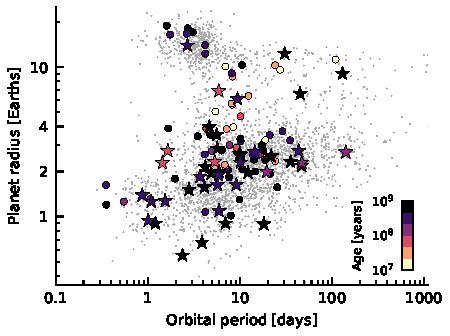
\includegraphics[width=0.7\textwidth]{rp_vs_period_scatter_20240415_colorbyage_showaux-gyro_anyyoung_anyyoung.pdf}
  \end{center}
  \vspace{-0.5cm}
  
  \caption{
    {\bf Sizes, orbital periods, and rotation-based ages of transiting
    exoplanets younger than one billion years.} Stars denote
    \nplyounggyrotwosigmanograzingnoruwe\ planets that are newly
    characterized in this work to have $t_{\rm gyro}$<1\,Gyr at
    $2$$\sigma$; circles are planets from the literature meeting the
    same age requirement, but with a heterogeneous set of age
    provenances.  Gray points are transiting planets from the NASA
    Exoplanet Archive older than 1\,Gyr.  If one were to select for
    precise ages ($t/\sigma_{\rm t}>3$), this would hide $\approx$ten
    $<$0.5\,Gyr planets, and add $\approx$fifteen 0.5-1\,Gyr planets.
    For this plot, we require our Kepler stellar hosts to have no
    quality flags raised, and for the planets to
    similarly no have quality flags raised. 
    \label{fig:rp_period_age_results}
  }
\end{figure*}

\subsubsection{Rotation vs.~Lithium Age Comparison}

We judged the consistency of the independent rotation and
lithium-based ages by comparing the point-estimates of the posteriors,
when available.  There are three cases of interest:

\begin{enumerate}
  \item Two-sided posteriors available for both $t_{\rm gyro}$ and
    $t_{\rm Li}$: if their values were consistent within 2$\sigma$, we
    judged them to be consistent; if they were consistent within
    2-3$\sigma$, we suggest them to be ``maybe'' consistent.
    Otherwise, they are in disagreement.
    %
  \item If $t_{\rm Li}$ is a lower limit, we compare the $t_{\rm Li}$
    lower limit with the $1\sigma$ upper limit from $t_{\rm gyro}$; if
    the two overlapped, we judge the age estimates to be consistent.
    %
  \item If $t_{\rm Li}$ provides a two-sided posterior, and no
    rotation is reported, we judge the age estimates to be
    inconsistent.  This is because this lithium constraint can only be
    provided for G and K stars $\lesssim$2\,Gyr old, and Kepler should
    have been sensitive to the rotation periods of such stars.
\end{enumerate}

In the entire sample, this yielded \allagesyesconsistent\ consistent
cases, \allagesmaybeconsistent\ ``maybe'' cases, and
\allagesnoconsistent\ inconsistent.  Restricting our attention to the
$\lesssim$1\,Gyr stars, for which lithium ages are more constraining,
the respective counts are \minageltonegyryesconsistent,
\minageltonegyrmaybeconsistent, and \minageltonegyrnoconsistent.
Rephrased, in the overall sample, \fracconsistentallages\% of stars
have consistent rotation and lithium-based ages
(\fracpotentiallyconsistentallages\% potentially consistent).  In the
sample of sub-gigayear stars, \fracconsistentminageltonegyr\% of the
ages are consistent (\fracpotentiallyconsistentminageltonegyr\%
potentially consistent).  We feel it necessary to distinguish
``maybe'' consistent cases because of lingering uncertainties in how
the dispersion of the lithium data evolve over the first gigayear.  In
Appendix~\ref{app:inconsistent}, we discuss the
\minageltonegyrnoconsistent\ discrepant sub-gigayear stars in detail.


\subsubsection{New Young Systems}
%
Whenever both rotation and lithium find a star to be in a
narrowly-constrained age range, confidence in the true age greatly
increases, due to the independence of the two measurement techniques.
The empirical precision for the inferred ages as a function of $P_{\rm
rot}$, $EW_{\rm Li}$, and $T_{\rm eff}$ has been mapped out by
\citet{Bouma_2023} and \citet{Jeffries_2023} for rotation and lithium
respectively.  The region of greatest overlap is dictated by the
timescale for lithium depletion: for stars with temperatures between
4500-5500\,K with ages $\lesssim$500\,Myr, we can hope to obtain
independent two-sided constraints.

The youth of most of these systems, to our knowledge, is being
well-constrained for the first time in this work.  Here we limit
discussion to systems with $t_{\rm gyro}$$<$500\,Myr not in the clusters
mentioned above.

The new young planets
include five 1.8-3.8\,$R_\oplus$ mini-Neptunes
(Kepler-1529b $\approx$100\,Myr,
-1521b $\approx$195\,Myr,
-1467b $\approx$235\,Myr,
-955b $\approx$400\,Myr, and
-523b $\approx$440\,Myr),
a single Neptune-sized planet
(Kepler-971b $\approx$335\,Myr),
five 1.1-1.8\,$R_\oplus$ super-Earths
(Kepler-1930b $\approx$150\,Myr,
-1313b $\approx$185\,Myr,
-1565b $\approx$205\,Myr,
-1532b $\approx$400\,Myr,
-1481b $\approx$400\,Myr),
and three Earth or sub-Earth-sized planets
(Kepler-1933b $\approx$300\,Myr,
-1561b $\approx$420\,Myr,
-1482b $\approx$490\,Myr).
All of these planets are on orbital periods below 50\,days.

Of these planets, one specific highlight is Kepler-1933b, a 4.9\,day
1.0\,$R_\oplus$ Earth-sized planet.  Its rotation-based age of
$304^{+96}_{-112}$\,Myr agrees within $1\sigma$ of its lithium age,
though at half the relative uncertainty.  Based on these lines of
evidence, this system may be the youngest Earth-sized planet known,
comparable to systems such as HD~63433d \citep[1.1\,$R_\oplus$,
$414\pm23$\,Myr][]{2024AJ....167...54C}.

A less clear case is Kepler-447b, which is supposedly a 32\,$R_\oplus$
planet on a 7.8\,day grazing orbit.  Rotation and lithium independently
find a 420-440\,Myr age.  {\it LGB TODO What is up with the size?}.

%  Kepler-1529b, a 5.3\,day 2.0\,$R_\oplus$ mini-Neptune is $\approx$100\,Myr old.
%  Kepler-1930b, a 13.0\,day 1.5\,$R_\oplus$ super-Earth on a grazing orbit is $\approx$120-180\,Myr old.
%  Kepler-1313b, doubly unlucky, a 3.8\,day 1.7\,$R_\oplus$ super-Earth on a grazing orbit is $\approx$185\,Myr old.
%  Kepler-1521b, a 47.2\,day 2.3\,$R_\oplus$ mini-Neptune is 180-210\,Myr old.
%  Kepler-1467b, a 47.1\,day 3.1\,$R_\oplus$ mini-Neptune is 230-240\,Myr old.
%  Kepler-1565b, a 1.5\,day 1.3\,$R_\oplus$ super-Earth is 180-230\,Myr old.
%  Kepler-971b, a 9.6\,day 3.9\,$R_\oplus$ Neptune-sized planet is 300-370\,Myr old.
%  
%  Kepler-1933b is a 4.9\,day 1.0\,$R_\oplus$ Earth-sized planet.  Its
%  rotation-based age of $304^{+96}_{-112}$\,Myr agrees within $1\sigma$ of
%  its lithium age, though at half the relative uncertainty.  Based on
%  these lines of evidence, this system may be the youngest Earth-sized
%  planet known, comparable to systems such as HD~63433d
%  \citep[1.1\,$R_\oplus$, $414\pm23$\,Myr][]{2024AJ....167...54C}.
%  
%  Kepler-1532b is a 1.1\,day 1.3\,$R_\oplus$ super-Earth.  Rotation points to a $\approx$400\,Myr age, and lithium is consistent.
%  Kepler-955b is a 14.5\,day 2.7\,$R_\oplus$ mini-Neptune.  Rotation points to a $\approx$400\,Myr age, and lithium is consistent.
%  Kepler-1481b, a 5.9\,day 1.1\,$R_\oplus$ super-Earth has a
%  rotation-based age of $\approx$400\,Myr, and a $2\sigma$ lithium
%  detection that, upon visual inspection of the spectrum, is
%  believeable.  The implied lithium age is marginally consistent with
%  the rotation-based age, although perhaps with some tension.
%  Kepler-447b is supposedly a 32\,$R_\oplus$ planet (grazing) on a
%  7.8\,day grazing orbit.  Rotation and lithium independently find a
%  420-440\,Myr age.
%  Kepler-1561b is a 0.9\,$R_\oplus$ sub-Earth, on a 1.0\,day orbit.
%  Rotation points to a 420\,Myr age.  The detected EW$_{\rm Li}$ is
%  consistent, although given the star's temperature, not particularly
%  constraining.
%  The same is true for the 1.9\,$R_\oplus$ and 5.8\,day super-Earth Kepler-523b, and the 
%  1.0\,$R_\oplus$, 12.2\,day Earth-sized Kepler-1482b.


%\subsubsection{Need spectra}
%Kepler-1938...
%Kepler-762... (a HJ!)
%Kepler-1320



\section{Discussion}
\label{sec:disc}

\subsection{The Thin Disk's Star Formation History}

Zasowski et al fitted a chemical-isochrone model to APOGEE, X, Y, Z
data and presented a model for the star formation history of the MW.
The gist is a spike at z=2, and a gradual decrease since then, by
about a few of ten.

Mor2019 did isochrone fitting to Gaia, and found the same, but with a
spike at 3Gyr.

Our inferred gyro-age distribution of the Kepler field seems to agree
with these pictures.  The main value added is likely over the first
gigayear.

% compare against Berger+20, 
% note their sentence
% "Encouragingly, the distribution also qualita- tively matches the red giant asteroseismology-derived age distributions in Silva Aguirre et al. (2018) and Pinsonneault et al. (2018), as well as the rotation-based ages in Claytor et al. (2020) and the Galactic Archaeology with HERMES–Gaia ages in Buder et al. (2019)."
%
% also compare against Mor2019 and their literature assessment
% "Our findings that the thin disc SFH does not follow a sim- ple decreasing shape until the present are in good agreement with Snaith et al. (2015), and Haywood et al. (2016, 2018) who found, using data with metallicities and assuming a fixed IMF, the existence of an SFR quenching followed by a reactivation. Kroupa (2002a), using stellar kinematics, found the SFH to behave similarly. The relative maximum of the SFR that we find at 2–3 Gyr ago is compatible with the results of Vergely et al. (2002) and Cignoni et al. (2006) that, using Hipparcos data in a sphere of 80 pc around the Sun and assuming a fixed IMF, found maximum peaks at 1.75–2 Gyr ago and 2–3 Gyr ago, respec- tively. Recently, Bernard (2018), in a tentative work using TGAS data, pointed towards the existence of a relative maximum also located 2–3 Gyr ago."


%\subsection{Isochrone Age Comparison}

%\subsection{Lithium Age Comparison}

\subsection{Caveats}

\subsection{Future Directions}

%   \subsubsection{Evolutionary trends in time}
%   
%   {\it Kelvin-Helmholtz cooling}
%   $R_p \propto t^{-0.1}$ scaling \citep{Gupta_2019}
%   
%   {\it Early carving of the photoevaporation desert}
%   \citep{Owen_Lai_2018}
%   
%   {\it Rapidly decreasing abundance of big puffy planets}
%   Kepler not enough?
%   
%   {\it Mini-Neptunes turning into Super-Earths}
%   \citep[e.g.][]{Rogers_2021}
%   
%   {\it Boundary of the Super-Earth population moving up in time}
%   \citep{David_2021}




\section{Conclusions}
\label{sec:conclusions}

We began this article by asking two questions: how wrong is the assumption
of a uniform age distribution for stars in the galactic thin disk?
And why are only $\approx$50 sub-gigayear transiting planets
known, rather than the $\approx$500 that would be expected under the 
assumption of a uniform star formation history for
the $\approx$5{,}000 known planets?

In an attempt to answer these questions, we curated a sample of rotation
periods, lithium equivalent widths, and stellar temperatures using a combination
of archival and new data.
We derived new ages using empirical interpolation-based age scales
that have been calibrated against the latest available open cluster data.

Our analysis blindly recovered all 14 known Kepler planets in
clusters, with ages in agreement with the more precise cluster-based ages.
Although lithium provided only marginal added information for most of
the sample, the independent lithium and rotation ages agreed for
$\approx$90\% of cases.  In particular, we reported 
14 confirmed $<$500\,Myr planets
with strong age
constraints from both rotation and lithium, including five mini-Neptunes, five super-Earths,
three Earths and sub-Earths, and a Neptune-sized planet.

With respect to our original questions, we have 
three main conclusions.
\begin{enumerate}
  %FIXME: 120 number
  \item From the rotation rates of Kepler planet-hosting stars, we
    have identified  \nplyounggyrotwosigma\ planets younger than
    1\,Gyr at 2$\sigma$, and \nplyounggyro\ planets with median ages
    below 1\,Gyr.
    This implies that there are now $\approx$120-170 known
    sub-gigayear planets with well-constrained ages.
  %
  \item The age distributions of both the Kepler
    target stars and the known Kepler planet-hosts shows a
    demographic cliff.  
    There are \ratioobtoybstars\ times as many ``old'' (2-3\,Gyr)
    stars in the Kepler field as ``young'' (0-1\,Gyr) stars.
    The star formation rate today is \ratiosfr$\pm$\uncratiosfr\ times
    lower than it was three billion years ago.
  %
  \item The implication of the latter age distribution is that rather
    than expecting $\approx$500 sub-gigayear exoplanets, we should
    instead expect $\approx$250.
    We have therefore gone from a factor of ten discrepancy to a
    factor of at most two.
%    The issue is therefore mostly, although perhaps not entirely, resolved.
%    Some of the remaining missing young
%    transiting planets may be in the Kepler data.  Many more are
%    likely in K2 and TESS.
\end{enumerate}


% 4 CepHer, 2 MELANGE3, 6 Theia520, 2 NGC6811.




\acknowledgements
This work was supported by the 
Heising-Simons 51~Pegasi~b Fellowship (LGB)
and the Arthur R.~Adams SURF Fellowship (EKP).

(author contribution statements will go here)
L.G.B.~conceived the project, collected data, 
inferred ages, and wrote the manuscript.
E.K.P.~contributed to early iterations of the rotation-based age analysis.
L.A.H.~contributed to project design.
H.I. and A.W.H~contributed to acquisition, reduction, and analysis of
the HIRES data.
All authors assisted in manuscript revision.


\facilities{
  Gaia \citep{Gaia_DR3_2022},
  Kepler \citep{Borucki10},
  Keck:I (HIRES).
%  TESS \citep{ricker_transiting_2015},
%  NGTS \citep{Wheatley_2018}
}

\software{
    astropy \citep{Astropy18},
    matplotlib \citep{matplotlib},
    numpy \citep{numpy},
    scipy \citep{scipy},
}

\clearpage 

\startlongtable
\begin{deluxetable*}{llllllllrrrrrrl}
  %\tabletypesize{\footnotesize}
  \tabletypesize{\scriptsize}
  \tablecaption{Ages of Kepler planets and planet candidates.  This
  version of the table is truncated to include only the youngest confirmed Kepler planets,
  sorted by the minimum of either the rotation or lithium-based
  age.  The
  full machine-readable table contains ages and age limits for
  \nnonfopkoissomeageinfo\ non-false positive KOIs with MES$>$10.  
  A shell script to decode the $Q_{\rm gyro}$ quality flag is {\bf \href{https://gist.github.com/lgbouma/20368253f1a98da1b39cf32fdda0be13}{available online}}.
  \label{tab:planets}}
  %\toprule
  %\midrule
  %\endhead
  \startdata
  KOI & Kepler &  $T_{\rm eff}$ & $P_{\rm rot}$ & EW$_{\rm Li}$ &
  $t_{\rm gyro}$ & $t_{\rm Li} $ & Consistent? & $R_{\rm p}$ & $P_{\rm orb}$ &
  $Q_{\rm planet}$ & $Q_{\rm gyro}$ &  Spec? & Comment \\
  -- &   -- & K & days & m\AA & Myr & Myr &  str &   Earths &    days &       int  & int & bool & -- \\
  \hline
  K05245.01 & Kepler-1627 b & 5357 & 2.62 & $225\pm7$ & $80^{+152}_{-56} $ & $51^{+38}_{-27}$ & Yes & 3.79 & 7.2 & 0 & 1152 & 1 & Cep-Her \\
K07368.01 & Kepler-1974 b & 5068 & 2.56 & $248\pm4$ & $88^{+176}_{-64} $ & $54^{+47}_{-25}$ & Yes & 2.22 & 6.84 & 0 & 1536 & 1 & Cep-Her \\
K06228.01 & Kepler-1644 b & 5521 & 1.43 & $-2\pm13$ & $72^{+144}_{-48} $ & $> 767$ & No & 1.88 & 21.09 & 4 & 1666 & 1 & Unres. Binary \\
K06186.01 & Kepler-1643 b & 4918 & 5.05 & $120\pm6$ & $80^{+176}_{-56} $ & $191^{+92}_{-76}$ & Yes & 2.11 & 5.34 & 0 & 2048 & 1 & Cep-Her \\
K03933.01 & Kepler-1699 b & 5496 & 4.16 & $-11\pm7$ & $80^{+104}_{-56} $ & $> 889$ & No & 1.32 & 3.49 & 0 & 1152 & 1 & Unres. Binary \\
K03916.01 & Kepler-1529 b & 4974 & 6.43 & $200\pm6$ & $104^{+112}_{-72} $ & $90^{+53}_{-39}$ & Yes & 2.01 & 5.34 & 0 & 2048 & 1 & \checkmark \checkmark \\
K07913.01 & Kepler-1975 b & 4450 & 3.36 & $56\pm9$ & $96^{+216}_{-72} $ & $> 57$ & Yes & 2.03 & 24.28 & 0 & 1792 & 1 & Cep-Her \\
K01804.01 & Kepler-957 b & 4947 & 4.52 & $24\pm9$ & $96^{+192}_{-72} $ & $> 241$ & Yes & 6.9 & 5.91 & 0 & 0 & 1 & \checkmark \\
K03936.02 & Kepler-1930 b & 4906 & 7.1 & $170\pm4$ & $176^{+104}_{-64} $ & $115^{+55}_{-49}$ & Yes & 1.52 & 13.03 & 4 & 0 & 1 &  \\
K03876.01 & Kepler-1928 b & 5577 & 4.64 & $137\pm4$ & $144^{+104}_{-88} $ & $189^{+150}_{-94}$ & Yes & 1.86 & 19.58 & 0 & 1024 & 1 & MELANGE-3 \\
K04069.01 & Kepler-1938 b & 4617 & 7.82 & $6\pm16$ & $152^{+112}_{-40} $ & $> 208$ & Yes & 1.47 & 13.06 & 0 & 1024 & 1 & \checkmark \\
K02678.01 & Kepler-1313 b & 5236 & 6.13 & $142\pm3$ & $192^{+112}_{-88} $ & $174^{+96}_{-72}$ & Yes & 1.71 & 3.83 & 4 & 1024 & 1 &  \\
K04194.01 & Kepler-1565 b & 4958 & 7.4 & $133\pm7$ & $232^{+104}_{-88} $ & $174^{+81}_{-72}$ & Yes & 1.27 & 1.54 & 0 & 0 & 1 & \checkmark \checkmark \\
K03835.01 & Kepler-1521 b & 4806 & 7.82 & $117\pm5$ & $208^{+96}_{-72} $ & $176^{+79}_{-69}$ & Yes & 2.3 & 47.15 & 0 & 1024 & 1 & \checkmark \checkmark \\
K01838.01 & Kepler-970 b & 4314 & 9.23 & $36\pm14$ & $176^{+120}_{-40} $ & $> 92$ & Yes & 2.15 & 16.74 & 4 & 0 & 1 & MELANGE-3 \\
K00063.01 & Kepler-63 b & 5486 & 5.49 & $89\pm4$ & $224^{+96}_{-96} $ & $542^{+475}_{-256}$ & Yes & 5.64 & 9.43 & 0 & 2048 & 1 & \checkmark \checkmark \\
K01199.01 & Kepler-786 b & 4680 & 33.06 & $83\pm6$ & $3872^{+96}_{-168} $ & $228^{+168}_{-87}$ & No & 2.31 & 53.53 & 0 & 0 & 1 & Mystery \\
K03316.01 & Kepler-1467 b & 5252 & 6.31 & $122\pm6$ & $232^{+112}_{-104} $ & $236^{+151}_{-95}$ & Yes & 3.11 & 47.06 & 0 & 0 & 1 & \checkmark \checkmark \\
K01074.01 & Kepler-762 b & 5921 & 4.01 & $-27\pm25$ & $240^{+112}_{-96} $ & $> 548$ & Maybe & 15.19 & 3.77 & 0 & 2560 & 1 &  \\
K01839.01 & Kepler-971 b & 5447 & 6.22 & $105\pm6$ & $305^{+96}_{-112} $ & $366^{+290}_{-164}$ & Yes & 3.93 & 9.59 & 0 & 128 & 1 &  \\
K01833.01 & Kepler-968 b & 4413 & 10.46 & $10\pm18$ & $329^{+104}_{-88} $ & $> 159$ & Yes & 1.85 & 3.69 & 0 & 0 & 1 & Theia-520 \\
K01833.03 & Kepler-968 c & 4413 & 10.46 & $10\pm18$ & $329^{+104}_{-88} $ & $> 159$ & Yes & 1.63 & 5.71 & 0 & 0 & 1 & Theia-520 \\
K01833.02 & Kepler-968 d & 4413 & 10.46 & $10\pm18$ & $329^{+104}_{-88} $ & $> 159$ & Yes & 2.28 & 7.68 & 4 & 0 & 1 & Theia-520 \\
K00775.02 & Kepler-52 b & 4164 & 11.85 & $22\pm18$ & $353^{+184}_{-88} $ & $> 100$ & Yes & 2.19 & 7.88 & 0 & 0 & 1 & Theia-520 \\
K00775.01 & Kepler-52 c & 4164 & 11.85 & $22\pm18$ & $353^{+184}_{-88} $ & $> 100$ & Yes & 2.04 & 16.38 & 0 & 0 & 1 & Theia-520 \\
K00775.03 & Kepler-52 d & 4164 & 11.85 & $22\pm18$ & $353^{+184}_{-88} $ & $> 100$ & Yes & 2.03 & 36.45 & 0 & 0 & 1 & Theia-520 \\
K02675.01 & Kepler-1312 b & 5584 & 6.13 & $86\pm4$ & $361^{+72}_{-112} $ & $642^{+617}_{-318}$ & Yes & 2.07 & 5.45 & 0 & 2048 & 1 & \checkmark \checkmark \\
K02675.02 & Kepler-1312 c & 5584 & 6.13 & $86\pm4$ & $361^{+72}_{-112} $ & $642^{+617}_{-318}$ & Yes & 0.94 & 1.12 & 0 & 2048 & 1 & \checkmark \checkmark \\
K04004.01 & Kepler-1933 b & 5576 & 6.21 & $85\pm3$ & $369^{+72}_{-112} $ & $642^{+603}_{-318}$ & Yes & 1.01 & 4.94 & 4 & 0 & 1 &  \\
K02174.03 & Kepler-1802 b & 4245 & 11.45 & -- & $377^{+200}_{-104} $ & -- & -- & 1.71 & 7.73 & 4 & 308 & 0 &  \\
K02174.02 & Kepler-1802 c & 4245 & 11.45 & -- & $377^{+200}_{-104} $ & -- & -- & 2.05 & 33.14 & 0 & 308 & 0 &  \\
K03935.01 & Kepler-1532 b & 5554 & 6.48 & $90\pm6$ & $401^{+64}_{-104} $ & $567^{+545}_{-278}$ & Yes & 1.26 & 1.09 & 0 & 0 & 1 & \checkmark \checkmark \\
K01801.01 & Kepler-955 b & 5221 & 7.5 & $79\pm4$ & $401^{+96}_{-136} $ & $536^{+481}_{-237}$ & Yes & 2.69 & 14.53 & 0 & 0 & 1 & \checkmark \checkmark \\
K01800.01 & Kepler-447 b & 5648 & 6.4 & $103\pm3$ & $417^{+64}_{-72} $ & $405^{+355}_{-203}$ & Yes & 18.49 & 7.79 & 4 & 1024 & 1 &  \\
K03370.02 & Kepler-1481 b & 4832 & 9.11 & $22\pm7$ & $409^{+120}_{-120} $ & $> 210$ & Yes & 1.09 & 5.94 & 0 & 0 & 1 & \checkmark \\
K04156.01 & Kepler-1943 b & 6002 & -- & $99\pm5$ & -- & $409^{+520}_{-254}$ & No & 1.29 & 4.85 & 4 & 518 & 1 &  \\
K00448.01 & Kepler-159 b & 4511 & 10.5 & $19\pm10$ & $417^{+160}_{-112} $ & $> 161$ & Yes & 2.3 & 10.14 & 0 & 2048 & 1 & \checkmark \\
K00448.02 & Kepler-159 c & 4511 & 10.5 & $19\pm10$ & $417^{+160}_{-112} $ & $> 161$ & Yes & 2.75 & 43.59 & 0 & 2048 & 1 & \checkmark \\
K00046.01 & Kepler-101 b & 5498 & -- & $100\pm5$ & -- & $419^{+349}_{-196}$ & No & 5.9 & 3.49 & 0 & 518 & 1 &  \\
K04169.01 & Kepler-1561 b & 5742 & 6.18 & $66\pm3$ & $425^{+72}_{-72} $ & $1409^{+1718}_{-788}$ & Maybe & 0.94 & 1.01 & 0 & 1024 & 1 & \checkmark \checkmark \\
K02708.01 & Kepler-1320 b & 4536 & 10.46 & $25\pm32$ & $425^{+168}_{-104} $ & $> 140$ & Yes & 1.39 & 0.87 & 0 & 0 & 1 & \checkmark \\
K00119.01 & Kepler-108 b & 5626 & -- & $100\pm5$ & -- & $438^{+402}_{-220}$ & No & 8.2 & 49.18 & 0 & 418 & 1 &  \\
K00119.02 & Kepler-108 c & 5626 & -- & $100\pm5$ & -- & $438^{+402}_{-220}$ & No & 7.78 & 190.32 & 4 & 418 & 1 &  \\
K00323.01 & Kepler-523 b & 5267 & 7.6 & $49\pm4$ & $441^{+88}_{-112} $ & $1824^{+2706}_{-1047}$ & Maybe & 1.9 & 5.84 & 0 & 0 & 1 & \checkmark \checkmark \\
K02115.01 & Kepler-67 b & 5126 & 10.39 & $83\pm10$ & $882^{+104}_{-120} $ & $458^{+451}_{-206}$ & Yes & 2.96 & 15.73 & 0 & 0 & 1 & \checkmark \checkmark \\
K00002.01 & Kepler-2 b & 6436 & -- & $83\pm4$ & -- & $485^{+924}_{-353}$ & -- & 16.42 & 2.2 & 0 & 7 & 1 &  \\
K03371.02 & Kepler-1482 b & 5330 & 7.7 & $52\pm3$ & $489^{+80}_{-88} $ & $1630^{+2285}_{-904}$ & Maybe & 1.0 & 12.25 & 0 & 640 & 1 &  \\
K03010.01 & Kepler-1410 b & 3808 & 14.19 & $-21\pm24$ & $489^{+545}_{-168} $ & $> 80$ & Yes & 1.39 & 60.87 & 0 & 0 & 1 & \checkmark \\
K03497.01 & Kepler-1512 b & 4894 & 9.33 & $14\pm8$ & $505^{+136}_{-112} $ & $> 295$ & Yes & 0.8 & 20.36 & 4 & 2690 & 1 &  \\
K03864.01 & Kepler-1698 b & 4866 & 9.49 & $2\pm8$ & $521^{+144}_{-120} $ & $> 358$ & Yes & 0.9 & 1.21 & 0 & 0 & 1 & \checkmark \\
K05447.02 & Kepler-1629 b & 5585 & 7.45 & -- & $529^{+64}_{-64} $ & -- & -- & 0.67 & 3.88 & 0 & 0 & 0 &  \\
K01779.01 & Kepler-318 b & 5799 & 7.09 & $65\pm3$ & $561^{+104}_{-72} $ & $1507^{+1876}_{-858}$ & Yes & 3.97 & 4.66 & 0 & 0 & 1 & \checkmark \checkmark \\
K01779.02 & Kepler-318 c & 5799 & 7.09 & $65\pm3$ & $561^{+104}_{-72} $ & $1507^{+1876}_{-858}$ & Yes & 3.1 & 11.82 & 4 & 0 & 1 &  \\
K03324.01 & Kepler-1469 b & 5356 & 8.15 & $-5\pm25$ & $561^{+72}_{-80} $ & $> 535$ & Yes & 2.53 & 21.86 & 0 & 0 & 1 & \checkmark \\
K04246.01 & Kepler-1576 b & 5794 & 7.09 & $17\pm8$ & $561^{+96}_{-72} $ & $> 613$ & Yes & 0.9 & 6.98 & 0 & 2048 & 1 & \checkmark \\
K02035.01 & Kepler-1066 b & 5847 & 7.0 & $60\pm4$ & $585^{+152}_{-80} $ & $2018^{+2616}_{-1187}$ & Maybe & 1.96 & 1.93 & 4 & 0 & 1 &  \\
K02084.01 & Kepler-1792 b & 4942 & 9.49 & $13\pm11$ & $585^{+152}_{-136} $ & $> 312$ & Yes & 2.15 & 4.2 & 0 & 0 & 1 & \checkmark \\
K03274.01 & Kepler-1451 b & 5675 & 7.82 & $42\pm4$ & $593^{+80}_{-64} $ & $> 316$ & Yes & 2.33 & 35.62 & 0 & 0 & 1 & \checkmark \\
K01615.01 & Kepler-908 b & 5670 & 7.88 & $67\pm4$ & $601^{+80}_{-64} $ & $1317^{+1607}_{-724}$ & Yes & 1.36 & 1.34 & 0 & 2560 & 1 &  \\
K02022.01 & Kepler-349 b & 5756 & 7.71 & $64\pm6$ & $617^{+96}_{-72} $ & $1686^{+2185}_{-976}$ & Yes & 1.99 & 5.93 & 0 & 0 & 1 & \checkmark \checkmark \\
K02022.02 & Kepler-349 c & 5756 & 7.71 & $64\pm6$ & $617^{+96}_{-72} $ & $1686^{+2185}_{-976}$ & Yes & 1.97 & 12.25 & 0 & 0 & 1 & \checkmark \checkmark \\
K00620.01 & Kepler-51 b & 5635 & 8.14 & $48\pm8$ & $625^{+72}_{-64} $ & $> 258$ & Yes & 6.62 & 45.16 & 0 & 0 & 1 & \checkmark \\
K00620.03 & Kepler-51 c & 5635 & 8.14 & $48\pm8$ & $625^{+72}_{-64} $ & $> 258$ & Yes & 5.49 & 85.32 & 4 & 0 & 1 &  \\
K00620.02 & Kepler-51 d & 5635 & 8.14 & $48\pm8$ & $625^{+72}_{-64} $ & $> 258$ & Yes & 9.04 & 130.18 & 0 & 0 & 1 & \checkmark \\
K02803.01 & Kepler-1877 b & 5506 & 8.37 & $3\pm12$ & $625^{+64}_{-64} $ & $> 726$ & Maybe & 0.55 & 2.38 & 0 & 0 & 1 & \checkmark \\
K00720.04 & Kepler-221 b & 5070 & 9.3 & $21\pm5$ & $633^{+120}_{-112} $ & $> 341$ & Yes & 1.51 & 2.8 & 0 & 0 & 1 & \checkmark \\
K00720.01 & Kepler-221 c & 5070 & 9.3 & $21\pm5$ & $633^{+120}_{-112} $ & $> 341$ & Yes & 2.86 & 5.69 & 0 & 0 & 1 & \checkmark \\
K00720.02 & Kepler-221 d & 5070 & 9.3 & $21\pm5$ & $633^{+120}_{-112} $ & $> 341$ & Yes & 2.57 & 10.04 & 0 & 0 & 1 & \checkmark \\
K00720.03 & Kepler-221 e & 5070 & 9.3 & $21\pm5$ & $633^{+120}_{-112} $ & $> 341$ & Yes & 2.58 & 18.37 & 4 & 0 & 1 &  \\
K03097.02 & Kepler-431 b & 6259 & 16.16 & $80\pm3$ & -- & $671^{+1092}_{-458}$ & -- & 0.93 & 6.8 & 4 & 2055 & 1 &  \\
K03097.03 & Kepler-431 c & 6259 & 16.16 & $80\pm3$ & -- & $671^{+1092}_{-458}$ & -- & 0.93 & 8.7 & 4 & 2055 & 1 &  \\
K03097.01 & Kepler-431 d & 6259 & 16.16 & $80\pm3$ & -- & $671^{+1092}_{-458}$ & -- & 1.08 & 11.92 & 4 & 2055 & 1 &  \\
K01982.01 & Kepler-1781 b & 5363 & 9.17 & -- & $705^{+80}_{-72} $ & -- & -- & 1.95 & 4.89 & 0 & 0 & 0 &  \\
K01835.02 & Kepler-326 b & 5142 & 9.56 & $8\pm8$ & $721^{+112}_{-96} $ & $> 506$ & Yes & 1.25 & 2.25 & 0 & 640 & 1 &  \\
K01835.01 & Kepler-326 c & 5142 & 9.56 & $8\pm8$ & $721^{+112}_{-96} $ & $> 506$ & Yes & 1.38 & 4.58 & 0 & 640 & 1 &  \\
K01835.03 & Kepler-326 d & 5142 & 9.56 & $8\pm8$ & $721^{+112}_{-96} $ & $> 506$ & Yes & 1.31 & 6.77 & 0 & 640 & 1 &  \\
K03375.01 & Kepler-1918 b & 5522 & 9.11 & -- & $721^{+72}_{-72} $ & -- & -- & 2.19 & 47.06 & 0 & 0 & 0 &  \\
K01797.01 & Kepler-954 b & 4736 & 10.68 & $4\pm11$ & $729^{+216}_{-184} $ & $> 270$ & Yes & 2.16 & 16.78 & 0 & 0 & 1 & \checkmark \\
K03681.01 & Kepler-1514 b & 5852 & 7.87 & $69\pm2$ & $745^{+345}_{-128} $ & $1302^{+1622}_{-754}$ & Yes & 11.94 & 217.83 & 0 & 516 & 1 &  \\
K03681.02 & Kepler-1514 c & 5852 & 7.87 & $69\pm2$ & $745^{+345}_{-128} $ & $1302^{+1622}_{-754}$ & Yes & 1.17 & 10.51 & 4 & 516 & 1 &  \\
K01821.01 & Kepler-963 b & 5383 & 9.42 & -- & $745^{+80}_{-72} $ & -- & -- & 2.64 & 9.98 & 0 & 2048 & 0 &  \\
K00647.01 & Kepler-634 b & 6272 & -- & $77\pm3$ & -- & $768^{+1250}_{-527}$ & -- & 2.13 & 5.17 & 0 & 7 & 1 &  \\
K02037.01 & Kepler-1995 b & 4746 & 10.8 & $9\pm21$ & $770^{+216}_{-192} $ & $> 223$ & Yes & 3.46 & 73.76 & 0 & 2048 & 1 & \checkmark \\
K01781.02 & Kepler-411 b & 4920 & 10.32 & $4\pm3$ & $778^{+160}_{-168} $ & $> 396$ & Yes & 2.2 & 3.01 & 4 & 0 & 1 &  \\
K01781.01 & Kepler-411 c & 4920 & 10.32 & $4\pm3$ & $778^{+160}_{-168} $ & $> 396$ & Yes & 3.47 & 7.83 & 0 & 0 & 1 & \checkmark \\
K01781.03 & Kepler-411 d & 4920 & 10.32 & $4\pm3$ & $778^{+160}_{-168} $ & $> 396$ & Yes & 3.46 & 58.02 & 4 & 0 & 1 &  \\
K00001.01 & Kepler-1 b & 5730 & -- & $81\pm3$ & -- & $785^{+845}_{-419}$ & No & 14.04 & 2.47 & 4 & 0 & 1 &  \\
 %\\
% \rule
%  K07375.01 & -- & 4212 & 3.88 & $117\pm9$ & $104^{+235}_{-72}$ & $70^{+37}_{-21}$ & Yes & 1.73 & 4.85 & 0 & 2560 & 1 &  \\
K03991.01 & -- & 5226 & 5.22 & $98\pm3$ & $71^{+91}_{-48}$ & $354^{+253}_{-145}$ & Maybe & 1.37 & 1.57 & 0 & 2176 & 1 &  \\
K01546.01 & -- & 5639 & 0.9 & $33\pm24$ & $75^{+134}_{-51}$ & $> 316$ & Maybe & 11.92 & 0.92 & 0 & 2176 & 1 &  \\
K05482.01 & -- & 5519 & 0.81 & -- & $77^{+144}_{-53}$ & -- & -- & 2.96 & 31.71 & 4 & 2690 & 0 &  \\
K00064.01 & -- & 5306 & 2.23 & $3\pm4$ & $81^{+129}_{-55}$ & $> 567$ & No & 10.49 & 1.95 & 4 & 4614 & 1 &  \\
K06188.01 & -- & 5209 & 1.62 & $6\pm11$ & $84^{+171}_{-58}$ & $> 554$ & Maybe & 2.75 & 1.65 & 0 & 2048 & 1 &  \\
K02695.01 & -- & 5174 & 2.88 & -- & $86^{+176}_{-59}$ & -- & -- & 20.23 & 2.5 & 4 & 640 & 0 &  \\
K07449.01 & -- & 4928 & 1.31 & -- & $92^{+194}_{-63}$ & -- & -- & 20.43 & 1.32 & 4 & 2048 & 0 &  \\
K06130.01 & -- & 4560 & 3.02 & $-1\pm25$ & $94^{+217}_{-65}$ & $> 186$ & Yes & 1.45 & 1.54 & 0 & 2976 & 1 &  \\
K06195.01 & -- & 4677 & 1.42 & $-8\pm30$ & $94^{+210}_{-65}$ & $> 208$ & Yes & 2.28 & 1.44 & 0 & 2048 & 1 &  \\

  \enddata
  \tablecomments{``Confirmed'' planets appear in the machine-readable version before``candidate'' planets.
    The bit quality flags for the rotation-based ages,
    $Q_{\rm gyro}$, are described in Section~\ref{subsec:flags}.
    Concisely summarized, they are:
    Bit 0: $T_{\rm eff}/{\rm K} \in [ 3800-6200]$ ?
    Bit 1: $\log g$$<$4.2?
    Bit 2: $M_{\rm G}$<3.9 or $M_{\rm G}>8.5$?
    Bit 3: In KEBC?
    Bit 4: Large $d_{\rm xm,Kep-Gaia}$?
    Bit 5: Confused Kep-Gaia crossmatch?
    Bit 6: Gaia DR3 non-single star?
    Bit 7: RUWE$>$1.4?
    Bit 8: Crowded?
    Bit 9: Far from main-sequence?
    Bit 10: \citetalias{Santos_2021} CP/CB?
    Bit 11: $P_{\rm rot}$ not in the homogeneous
    \citetalias{Santos_2019} \citetalias{Santos_2021} sample?
    As an example, Kepler-1627 has $Q_{\rm gyro}$ flagged with bit 10 and bit 7.
    The analogous planet quality bit-flag, $Q_{\rm planet}$, has the
    following meaning.
    Bit 0: Candidate not reliable?
    Bit 1: MES$<$10?
    Bit 2: Grazing?
    For a star to have a high likelihood of being ``reliable for gyrochronology'' we suggest $Q_{\rm star}$ bits
    zero to nine to not be raised, and for a planet to be ``reliabe'', we suggested $Q_{\rm planet}$ to be zero.
  }
\end{deluxetable*}

\startlongtable
\begin{deluxetable*}{lllllllrrrrrr}
  \tabletypesize{\scriptsize}
  \tablecaption{
  Ages of Kepler target stars derived from rotation periods.  The
  full machine-readable table includes \nuniqstarsantosrot\ stars
  with reported rotation periods from \citetalias{Santos_2019} and
  \citetalias{Santos_2021}, \nuniqstarfinitegyroage\ of which have
  finite reported gyrochrone ages.  A random set of these stars is
  shown here to give an idea for form and content.  The quality
  bit-flag is as in Table~\ref{tab:planets}; requiring bits zero to
  nine to be null yields \nuniqstarsantosrotgyroappl\ stars for
  which gyrochronology is likely to be valid.  \label{tab:stars}}
  %\toprule
  %\midrule
  %\endhead
  \startdata
  KIC & Gaia DR3 &  $T_{\rm eff}$ & $P_{\rm rot}$ & $t_{\rm gyro}$ & $Q_{\rm gyro}$ \\
  -- &   -- & K & days &  Myr &    int  \\
  \hline
  8288455 & 2106058550991853312 & 4600 & 34.46 & $> 4000$ & 896 \\
9073955 & 2107145869211116800 & 6456 & 5.54 & -- & 5 \\
11559971 & 2129860714290473856 & 5307 & 22.09 & $2617^{+149}_{-134}$ & 0 \\
5178512 & 2101273686847355776 & 6595 & 10.02 & -- & 7 \\
11563886 & 2135020722359493376 & 4227 & 34.94 & $> 4000$ & 0 \\
12116739 & 2135236810754603136 & 5246 & 10.61 & $930^{+89}_{-94}$ & 0 \\
11199316 & 2134754743626117248 & 6085 & 11.12 & $2440^{+579}_{-688}$ & 128 \\
8455430 & 2079122650721924736 & 3516 & 24.54 & -- & 129 \\
8358143 & 2127110938787988864 & 5660 & 25.4 & $3646^{+218}_{-220}$ & 0 \\
7186851 & 2102573893706359936 & 5761 & 13.3 & $1693^{+437}_{-253}$ & 0 \\
 %\\
  %\hline
  \enddata
% \tablecomments{This table includes X, Y, Z... The machine-readable version,
%   available online, includes additional columns for .... 
% }
\end{deluxetable*}


\clearpage

\bibliographystyle{aasjournal}
\bibliography{bibliography}

\appendix
\section{Cases With Inconsistent Rotation and Lithium-Based Ages}
\label{app:inconsistent}

For Kepler-957, $T_{\rm eff}$=4947\,K, and $P_{\rm rot}$=4.52\,days,
This implies a rotation-based age of $96_{-72}^{+192}$\,Myr.  The
rotational broadening of the spectrum ($v\sin
i$$\approx$9.8$\pm$1.0\kms) is consistent with the nominal stellar
rotation period.  However, if this star were $\lesssim$500\,Myr old,
lithium should have been detectable at $>$50\,m\AA.  Lithium is
marginally if at all present in the spectrum ({\bf  EW$_{\rm
Li}$$<$XX\,m\AA at 2$\sigma$ }).  While the planet (nominally
6.9\,$R_\oplus$ on a 5.9\,day orbit) has been statistically validated
\citep{2016ApJ...822...86M}, inspecting the data validation reports this is
somewhat surprising.  The light curve shows greater scatter in-transit
than out of transit, appears near-grazing, and has a suggestion of a
strong odd-even depth difference.  This is a surprising system that
merits further attention.

% from inconsitent_tli_tgyro cases:
Kepler-1644 b
Kepler-1699 b
 Kepler-786 b

these have finite Li ages, but no rotation age (perhaps b/c of the missing prots...)
Kepler-1943 b
 Kepler-101 b
 Kepler-108 b
 Kepler-108 c
  Kepler-63 b
Kepler-1312 b
Kepler-1312 c
   Kepler-1 b

K02680.01
K02639.01



\section{Notable Individual Systems}

Kepler~221 is a 633$^{+120}_{-112}$\,Myr four-planet system.

Kepler~51 (CITE Masuda2014) has previously been noted for its bizarre architure.
The rotation-based age we find here is higher/lower than previously noted.

Kepler~411, a $\approx$780$\pm$170\,Myr early K dwarf with three
transiting planets at 3.0, 7.8, and 58\,days, has a rare
architecture.  \citet{2019A&A...624A..15S} conducted a transiting
timing analysis of the system, confirming Kepler-411d and arguing for
the presence of a fourth non-transiting planet, Kepler-411e, based on
the TTVs seen in Kepler-411d and assuming that the system is nearly
coplanar.  Regarding the stellar age, \citet{2019A&A...624A..15S} used
the \citet{2007ApJ...669.1167B} relation and the measured rotation
period, which yielded an estimate of 212$\pm$31\,Myr.  However, the
star's temperature ($\approx$4900\,K) puts it in a regime where the
\citeauthor{2007ApJ...669.1167B} relation has been known to not fit
observations for a while
\citep[e.g.][Fig.~9]{2008ApJ...687.1264M}.  Our adopted age of
$\approx$780$\pm$170\,Myr agrees with the open cluster calibrators.

%  Kepler-63b is interesting in that it is {\it missing} from our
%  catalog.  This 6.1\,$R_\oplus$ ``sub-Saturn'' has been shown to be in
%  a polar orbit based on both the Rossiter-McLaughlin effect and a
%  starspot-crossing analysis \citep{2013ApJ...775...54S}.  With $T_{\rm
%  eff}=5576\pm50$\,K, and a rotation period of 5.40\,days, we calculate
%  a rotation-based age of $t_{\rm gyro}$=$251^{+80}_{-90}$\,Myr,
%  qualitatively consistent with the estimates from
%  \citet{2013ApJ...775...54S}, though with larger uncertainties because
%  our age accounts for the intrinsic scatter in the open cluster
%  calibration sequences \citep{Bouma_2023}.  
%  While the usual catalogs (\citetalias{Santos_2019},
%  \citetalias{Santos_2021}, \citetalias{McQuillan_2014}, and
%  \citetalias{Mazeh_2015}) do not report this star's rotation period.
%  \citetalias{Santos_2021} flagged the system as ``potentially'' having
%  rotation-based modulation.


\section{Comparison Against Previous Literature Age Scales}
Searching the literature for gyrochronal analyses of the Kepler field,
the most relevant studies seemed to be those of
\citet{Walkowicz_2013}, \citet{Reinhold_2015}, and 
\citet{David_2021}.

Also Mathur2023, which does ``magneto-gyrochronology'', including the
Sph indicator in a model of the ages.


\subsection{Asteroseismic Age Comparison}
T Ceillier, J Van Saders et al 2016 MNRAS...



\section{Figure dump}

\begin{figure*}[!t]
  \begin{center}
    \leavevmode
    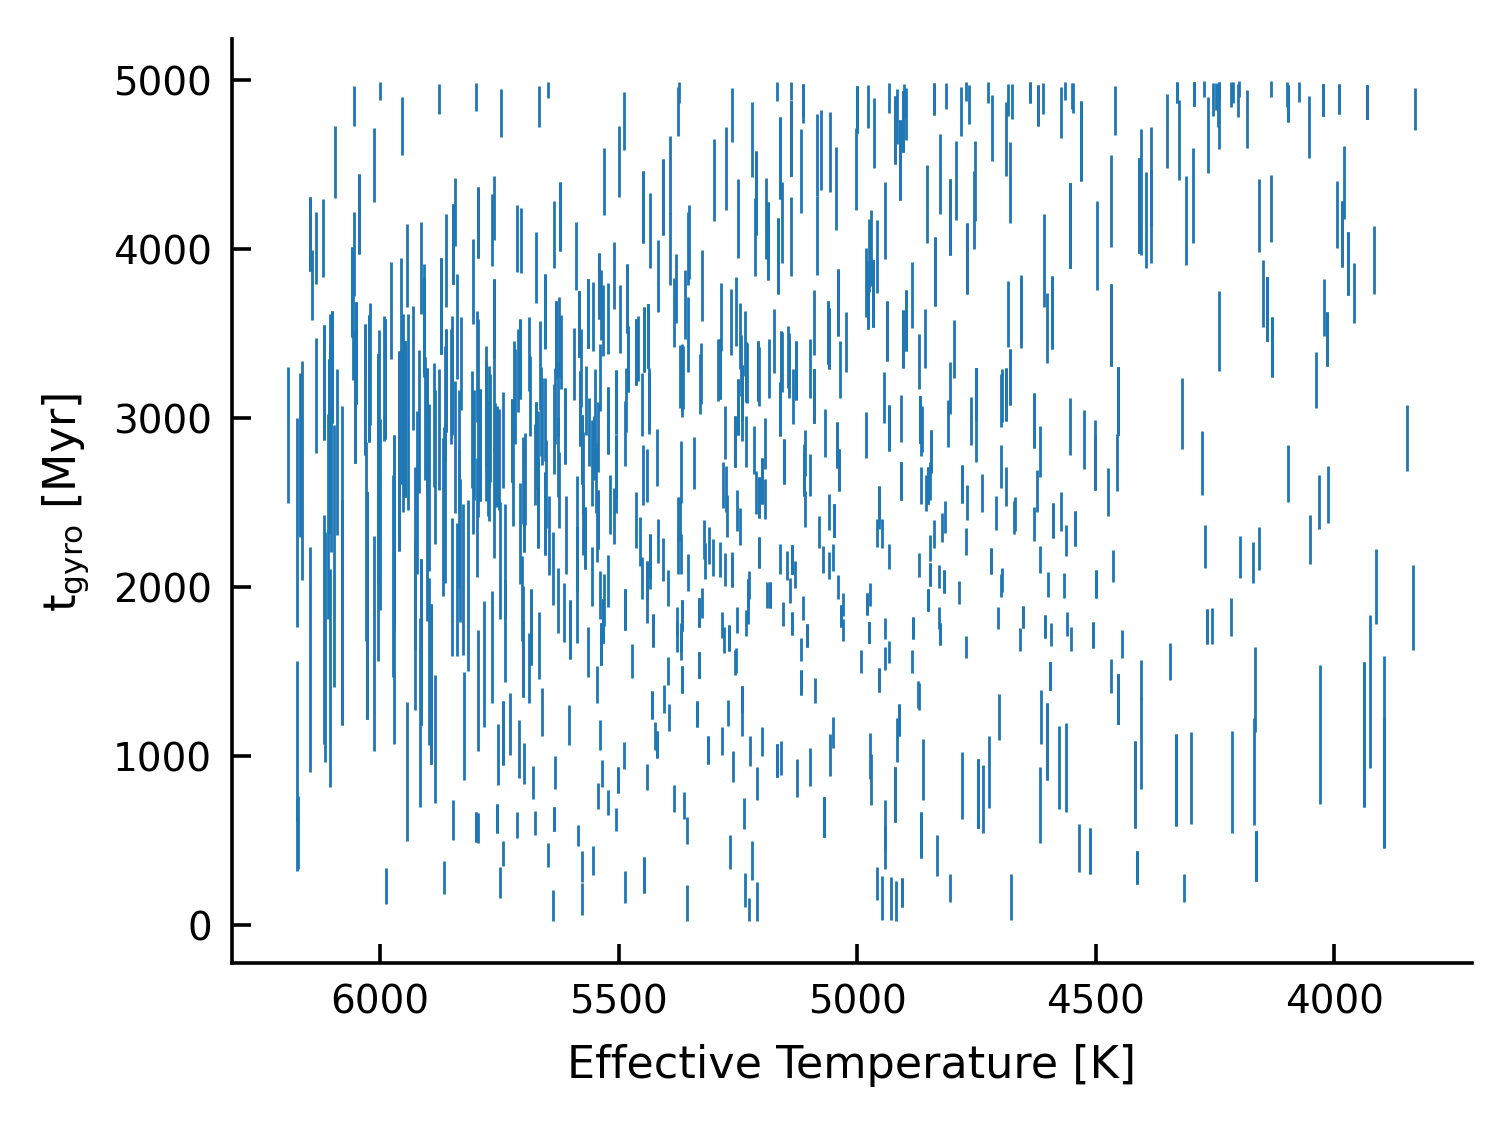
\includegraphics[width=0.5\textwidth]{gyroage_vs_teff_errs_showplanets_linear.png}
  \end{center}
  \vspace{-0.6cm}
  \caption{
    {\bf Gyro-age vs Teff}.
    $\pm$1$\sigma$ uncertainties are plotted around the median for Kepler stars (black) and KOIs (blue).
    Visual pileup on the left is b/c i) uncertain ages, and ii) lots of stars there.  Precision-land is the other portion.
    \label{fig:gyroage_vs_teff}
  }
\end{figure*}

\clearpage
\listofchanges

\end{document}
